%%%%%%%%%%%%%%%%%%%%%%% file template.tex %%%%%%%%%%%%%%%%%%%%%%%%%
%
% This is a general template file for the LaTeX package SVJour3
% for Springer journals.          Springer Heidelberg 2010/09/16
%
% Copy it to a new file with a new name and use it as the basis
% for your article. Delete % signs as needed.
%
% This template includes a few options for different layouts and
% content for various journals. Please consult a previous issue of
% your journal as needed.
%
%%%%%%%%%%%%%%%%%%%%%%%%%%%%%%%%%%%%%%%%%%%%%%%%%%%%%%%%%%%%%%%%%%%
%
% First comes an example EPS file -- just ignore it and
% proceed on the \documentclass line
% your LaTeX will extract the file if required
\begin{filecontents*}{example.eps}
%!PS-Adobe-3.0 EPSF-3.0
%%BoundingBox: 19 19 221 221
%%CreationDate: Mon Sep 29 1997
%%Creator: programmed by hand (JK)
%%EndComments
gsave
newpath
  20 20 moveto
  20 220 lineto
  220 220 lineto
  220 20 lineto
closepath
2 setlinewidth
gsave
  .4 setgray fill
grestore
stroke
grestore
\end{filecontents*}
%
\RequirePackage{fix-cm}
%
%\documentclass{svjour3}                     % onecolumn (standard format)
%\documentclass[smallcondensed]{svjour3}     % onecolumn (ditto)
\documentclass[smallextended]{svjour3}       % onecolumn (second format)
%\documentclass[twocolumn]{svjour3}          % twocolumn
%
\smartqed  % flush right qed marks, e.g. at end of proof
%
\usepackage{graphicx}
\usepackage{varwidth}
\usepackage{setspace}
\usepackage{perpage}
\usepackage{enumerate}
\MakePerPage{footnote}

\usepackage{tikz}
\usetikzlibrary{arrows,positioning,automata}
\usepackage[noend]{algpseudocode}
\usepackage{algorithm}
\usepackage{enumitem, kantlipsum}

\usepackage{times}

\usepackage{mathtools}
\usepackage{amssymb}

\usepackage{caption}

%
% \usepackage{mathptmx}      % use Times fonts if available on your TeX system
%
% insert here the call for the packages your document requires
%\usepackage{latexsym}
% etc.
%
% please place your own definitions here and don't use \def but
% \newcommand{}{}
%
% Insert the name of "your journal" with
% \journalname{myjournal}
%

\raggedbottom

\usepackage{atbegshi,picture}
%\usepackage{lipsum}

% \AtBeginShipout{\AtBeginShipoutUpperLeft{%
%   \put(\dimexpr\paperwidth-8.4cm\relax,-1.5cm){\makebox[0pt][r]{\framebox{SUBMITTED
%   TO IJSR. PLEASE DO NOT REDISTRIBUTE.}}}%
% }}

\begin{document}

\renewcommand{\labelitemi}{$\bullet$}

\algnewcommand\AND{\textbf{{\fontsize{10}{10}\selectfont AND}}}
\algnewcommand\OR{\textbf{{\fontsize{10}{10}\selectfont or}}}

\title{Toward Improving Human-Robot Collaboration with Emotional Awareness}%\thanks{Grants or
% other notes about the article that should go on the front page should be
%placed here. General acknowledgments should be placed at the end of the article.}
%}

%\subtitle{Do you have a subtitle?\\ If so, write it here}

%\titlerunning{Short form of title}        % if too long for running head

\author{Mahni Shayganfar \and
        Charles Rich \and
        Candace L. Sidner
}

%\authorrunning{Short form of author list} % if too long for running head

\institute{Mahni Shayganfar \and Charles Rich \and Candace L. Sidner \at
              100 Institute Road, Worcester, MA, USA 01609-2280 \\
              Tel.: +1 508-831-5357\\
              Fax: +1 508-831-5776\\
              \email{mshayganfar@wpi.edu}\\
              \email{rich@wpi.edu}\\
              \email{sidner@wpi.edu}\\
%             \emph{Present address:} of F. Author  %  if needed
}

\date{Received: date / Accepted: date}
% The correct dates will be entered by the editor


\maketitle

\begin{abstract}

Current computational theories used for human-robot collaboration specify the
structure of collaborative activities, but are weak on the underlying processes
that generate and maintain these structures. We argue that emotions are crucial
to these underlying processes and have developed a new computational theory,
called Affective Motivational Collaboration Theory, that combines emotion-based
processes, such as appraisal and coping, with collaboration processes, such as
planning, in a single unified framework. This work is implemented as part of a
larger effort to build robots capable of generating and recognizing emotions in
order to be better collaborators. We have investigated the mutual influences of
affective and collaborative processes in a cognitive theory to support
interaction between humans and robots or virtual agents. We build primarily on
the \textit{cognitive appraisal} theory of emotions and the \textit{SharedPlans}
theory of collaboration to investigate the structure, fundamental processes and
functions of emotions in a collaboration. We have developed new algorithms for
appraisal processes as part of a new overall computational model. We have
evaluated our implemented appraisal algorithms by conducting an online user
study.

% we have also developed a goal management algorithm based on a cost function that
% we use to choose the goal in the shared plan during collaboration.

\keywords{Human-Robot Collaboration \and Emotional Awareness \and Affective
Motivational Collaboration Theory}
% \PACS{PACS code1 \and PACS code2 \and more}
% \subclass{MSC code1 \and MSC code2 \and more}
\end{abstract}

\section{Introduction}
\label{intro}

A key aspect of the sociability of robots is their ability to collaborate with
humans in the same environment. Collaboration is a coordinated activity in which
the participants work jointly to satisfy a shared goal
\cite{grosz:plans-discourse}. There are many challenges in achieving a
successful collaboration between robots and humans. To meet these challenges, it
is crucial to understand what makes a collaboration not only successful, but
also efficient. Existing computational models of collaboration explain some of
the important concepts underlying collaboration; such as the presence of a
reason for collaborators' commitment, and the necessity of communicating about
mental states in order to maintain progress over the course of a collaboration.
The most prominent collaboration theories are based on plans and intentions
\cite{cohen:teamwork} \cite{grosz:plans-discourse}, and they support teamwork
and collaboration between humans and robots or virtual agents. However, these
theories explain only the structure of a collaboration. For instance, in
SharedPlans theory collaborators build a shared plan containing a collection of
beliefs and intentions about the actions in the plan. Collaborators communicate
these beliefs and intentions via utterances about actions that contribute to the
shared plan. This communication leads to the incremental construction of a
shared plan, and ultimately successful completion of the collaboration. In
contrast, in Joint Intentions theory, the notion of joint intention is viewed as
a persistent commitment of the team members to a shared goal. In this theory,
once an agent enters into a joint commitment with other agents, it should
communicate its private beliefs to other team members.

Although existing collaboration theories explain the important elements of a
collaboration structure, the underlying processes required to dynamically
create, use, and maintain the elements of this structure are largely
unexplained. For instance, a general mechanism has yet to be developed that
allows an agent to effectively integrate the influence of its collaborator's
perceived or anticipated emotions into its own cognitive mechanisms to prevent
shared task failures while maintaining collaborative behavior. Therefore, a
process view of collaboration must include certain key elements. It should
inherently involve social interactions since all collaborations occur between
social agents, and it should essentially constitute a means of modifying the
content of social interaction as the collaboration unfolds. The underlying
processes of emotions possess these two properties, and social functions of
emotions explain some aspects of the underlying processes in collaboration.
This work is implemented as part of a larger effort to build robots capable of
generating and recognizing emotions in order to be better collaborators.

Humans are emotional and social beings; emotions are involved in many different
social contexts including collaboration. Although there are purely personal
emotions, most emotions are experienced in a social context and acquire their
significance in relation to this context
\cite{parkinson:emotion-social-interaction}. For instance, humans are influenced
by the emotions of those around them. They also have emotions about the actions
of people around them. They have emotions about the events that occur in the
other people's lives. Also, humans' concern about their relationships with
others elicits emotion. They can feel emotion about their personal successes and
failures and those of others. Moreover, socially shared and regulated emotions
can provide social meanings to events happening in the environment
\cite{wisecup:sociology-emotions}.

There is also a communicative aspect of emotions. For instance, emotions are
often intended to convey information to others \cite{goffman:self-presentation}.
Emotions are also involved in verbal behaviors. For instance, an utterance can
include both content and relational meaning. An emotion might appear to be
elicited by the content of the utterance, but in fact be an individual's
response to the relational meaning \cite{planalp:communicating-emotion}. The
interpretation of these relational meanings are handled by the appraisal of
events. Appraisal processes give us a way to view emotion as social
\cite{hooft:sharing-emotions}. Meaning is created by an individual's social
experiences in the social world, and individuals communicate these meanings
through utterances. Consequently, the meaning of these utterances and the
emotional communication change the dynamic of social interactions. A successful
and effective emotional communication necessitates ongoing reciprocal
adjustments between interactants that can happen by interpreting each other's
behaviors \cite{parkinson:emotion-social-interaction}. This adjustment procedure
requires a baseline and an assessment procedure. While the components of the
collaboration structure, e.g., shared plan, provide the baseline,
emotion-related processes provide the assessment procedure.

Since collaboration is a type of social context, the social functions of
emotions are required for an agent to perform adequately in such an environment.
In this paper, first, we present two pairs of hypothetical interaction
scenarios. Each pair contrasts an emotionally-aware with an emotionally
ignorant\footnote{In our implementation, we always consider neutral emotion for
the emotionally ignorant cases. Therefore, any human's negative or positive
perceived emotion will be ignored by the robot and persumed as neutral emotion.}
robot interacting with a human in the same situation. These scenarios highlight
the necessity of giving robots the capacity to understand and regulate emotions,
as well as to provide emotion-driven responses. We then briefly introduce
Affective Motivational Collaboration Theory which explains the underlying
processes of emotions and collaboration. The emotion-aware examples show how the
mechanisms of this theory are involved in agreeing on a shared goal with a robot
(Section \ref{sec:exp1}), and delegating a new task to the robot (Section
\ref{sec:exp3}). The emotion ignorance examples are the same, except that the
robot always perceives human's negative or positive emotions as neutral, and
ignores the human's verbally or nonverbally expressed emotions. As we discussed
above, there are certain types of emotion-regulated mechanisms with which a
collaborative robot can modify and maintain a collaboration structure (e.g.,
shared plan). We explain these mechanisms and their corresponding operations in
Affective Motivational Collaboration Theory (see Section
\ref{sec:computational-framework}).

There are several appraisal models (e.g., EMA \cite{marsella:ema-process-model})
contributing in different applications such as social sciences, virtual agents,
and robotics. However, none of these models have focused on the appraisal
processes during collaboration. We believe appraisal plays a key role in
collaboration due to its regulatory and evaluative nature. Also, collaboration
induces some changes to underlying appraisal processes due to its unique nature.
A cognitive appraisal theory of collaboration is a contribution beyond existing
generic appraisal theories because collaboration involves several key properties
in structural and functional levels. Most collaborative situations involve
participants with different beliefs and capabilities; usually collaborators only
have partial knowledge of the process of accomplishing the collaborative
activities; collaborative plans are more than the sum of individual plans;
collaborators are required to maintain mutual (as well as private) beliefs about
their shared goal; they need to be able to communicate with others
effectively; they need to commit to the group activities; collaborators need
to commit to the success of others; they need to reconcile between commitments
to the existing collaboration and other activities; and they need to interpret
others’ actions and utterances in the collaboration context. For instance,
support, commitment, and responsiveness are prerequisites of collaborative
interaction that induce changes to required underlying processes. One of these
processes is appraisal which has a key evaluative role during collaboration.
We believe appraisal processes must consider factors related to the
collaborative environment, rather than considering only the robot's plan.
For instance, although the appraisal models mostly use utility to compute the
relevance of an event, we have found new cognitive components involved in
determining utility because of the influence of the collaboration. These
components, such as the recurrence of a belief by the human collaborator or the
influence of the human collaborator's perceived emotion on the robot's decisions
emphasize the fact that collaboration requires different procedures in appraisal
processes. In this paper, we provide the relevance, desirability, expectedness,
and controllability appraisals of an event in the collaboration context.
Finally, we provide the results from an online user study that we have conducted
to evaluate our appraisal algorithms.

\section{Related Work}
\label{sec:related-work}

The prominent collaboration theories are mostly based on plans and joint
intentions \cite{cohen:teamwork,grosz:plans-discourse}, and they were derived
from the BDI paradigm developed by Bratman \cite{bratman:intentions-plans} which
is fundamentally reliant on folk psychology \cite{ravenscroft:folk}. The two
theories, Joint Intentions \cite{cohen:teamwork} and SharedPlans
\cite{grosz:plans-discourse}, have been extensively used to examine and describe
teamwork and collaboration. The SharedPlans theory is a general theory of
collaborative planning which accommodates multi-level action decomposition
hierarchies, and allows the process of generating complete plans. The
SharedPlans theory shows how a group of collaborators can incrementally form and
execute a shared plan, and describes how a shared plan coordinates their
activities towards achieving a shared goal. Furthermore, SharedPlans theory
emphasizes that collaborative plans are an interleaving of collaborators' mutual
beliefs and intentions about the actions in the plan
\cite{grosz:planning-acting,grosz:collaboration,grosz:plans-discourse}. In
contrast, the Joint Intentions theory as another formal theory of collaboration
is based on the idea of individual and joint intentions to act as a team member.
In this theory, a joint intention is a shared commitment to perform an action
while in a group mental state. Joint Intentions theory describes how team
members can jointly act together by sharing mental states about their actions
while an intention is viewed as a commitment to perform an action
\cite{cohen:teamwork}.

There are many research focusing on different aspects of collaboration based on
different collaboration theories, i.e., SharedPlans, Joint Intentions, and
hybrid theories of collaboration, e.g., STEAM \cite{tambe:flexible-teamwork}.
Some of these works present algorithms and computational models in a
teamwork environment based on the underlying structure of the SharedPlans theory
\cite{lochbaum:collaborative-planning,lochbaum:plan-models,yen:cast,yin:knowledge-based-sharedplans},
and Joint Intentions theory
\cite{breazeal:humanoid-robots,mutlu:coordination-robot}. The hybrid teamwork
model, STEAM \cite{tambe:flexible-teamwork}, has also been successfully applied
to a variety of domains
\cite{kabil:coordination-mechanisms,kitano:robocup,marsella:robocup,scerri:robot-agent-person}.
All of the works presented in this section lack a systematic integration of
collaboration theories with some theories capable of describing underlying
collaboration processes. Therefore, they either do not explain the structure and
the underlying processes of collaboration, or their approach in either or both
of these views is application oriented. The collaboration structure of Affective
Motivational Collaboration Theory is based on the SharedPlans theory
\cite{grosz:planning-acting,grosz:collaboration,grosz:plans-discourse}, and it
focuses on the processes that generate, maintain and update this structure based
on mental states. COLLAGEN \cite{rich:collaboration-manager,rich:discourse} 
incorporates certain algorithms for discourse generation and interpretation, and
is able to maintain a segmented interaction history, which facilitates the
discourse between a human and a robot \cite{rickel:discourse-theory-dialogue}.
We use its latest incarnation, i.e., Disco, for our implementation.

Furthermore, there are some works focusing on the concepts of robot assistants
\cite{clancey:agent-assistants-collaboration}, or teamwork and its challenges in
cognitive and behavioral levels
\cite{nikolaidis:collaboration-joint-action,scerri:prototype-distributed-teams}.
Some researchers have an overall look at a collaboration concept at the
architectural level
\cite{esau:integrating-emotion-collaboration,garcia:collaboration-emotional-awareness,sofge:collaboration-humanoid-space}.
There are other concepts such as joint actions and commitments
\cite{grosz:intention-dynamics-collaboration}, dynamics of intentions during
collaboration \cite{levesque:acting-together} providing more depth in the
context of collaboration. Some of these works emphasize the applicability of
emotions in their architectures, and some others emphasize the collaborative
aspect of their robots. The applications of different prominent collaboration
theories show the importance and the applicability of these theories in robots
and collaborative systems. The following examples briefly review some of the
applications of artificial emotions and appraisal theory of emotions in robots
and autonomous agents.\\

\textbf{Applications of Artificial Emotions} -- There are many research areas,
including robotics and autonomous agents, that employ the structure and/or
functions of emotions in their work with a variety of motivations behind
modeling emotions \cite{wehrle:motivations-modeling-emotion}. Some of these
works are inspired by specific psychological theories, some are freely using the
concept of emotion without using the theoretical background in social sciences
\cite{urban:pecs}, and some are using a combination of concepts from the
psychological theories \cite{kiryazov:modeling-appraisal-pad}. We can also see
the application of emotion theories in designing companion robots, robots
capable of expressing emotions and social behaviors, as well as robots which can
convey certain types of emotion products, e.g., empathy
\cite{breazeal:expressive-behavior,paiva:emotion-modeling,shayganfar:methodology}.
Robots also use emotions theories for some other purposes such as automatic
affect recognition using different modalities \cite{zeng:affect-recognition},
and behavior adaptation \cite{liu:affect-robot-behavior}.

Furthermore, emotions have different intra/interpersonal functions. Motivation
is one of the crucial functions of emotions, since it can initiate, direct and
maintain goal-directed behaviors. The motivation mechanism in our work is
inspired by Murray's theory as well as Bach's approach on D$\ddot{o}$rner's
theory
\cite{bach:micropsi-agent-architecture,bach:psi,bach:motivaitional-system-ai,bach:next-generation-micropsi}.
It is focused on the role of emotion-driven motives in cognitive processes,
e.g., intention formation, during collaboration.\\

\textbf{Applications of Appraisal Theory} -- Appraisal theories of emotion were
first formulated by Arnold \cite{arnold:emotion-personality} and Lazarus
\cite{lazarus:emotion-adaptation} and then were actively developed in the early
80s by Ellsworth and Scherer and their students
\cite{roseman:appraisal-theory,sander:systems-approach-appraisal,scherer:nature-function-emotion,scherer:emotions-emergent,scherer:appraisal-processes}.
Computational appraisal models have been applied to a variety of uses including
contributions to psychology, robotics, AI, and HCI. For instance, Marsella and
Gratch have used EMA \cite{marsella:ema-process-model} to generate specific
predictions about how human subjects will appraise and cope with emotional
situations and argue that empirical tests of these predictions have implications
for psychological appraisal theory \cite{gratch:assessing-appraisal}. However,
EMA does not focus on the dynamics of collaborative contexts. There are several
examples in artificial intelligence and robotics of applying appraisal theory
\cite{adam:bdi-emotional-companion,kim:model-hri-appraisal,marsella:ema-process-model}.
In robotics, appraisal theory has been used to establish and maintain a better
interaction between a robot and a human
\cite{kim:model-hri-appraisal,sander:systems-approach-appraisal,vogiatzis:robot-museum}.
Appraisal theory has also been used in robots' decision making
\cite{castro:autonomous-robot-fear}, or in their cognitive systems
\cite{hudlicka:emotinos-reasons,marinier:emotion-reinforcement}. In the virtual
agents community, empathy and affective decision-making is a research topic that
has received much attention in the last decade
\cite{scott:modeling-empathy-agent,paiva:agent-care,pontier:women-robot-men,velasquez:emotions-motivations-agents}.

\section{Example Scenarios}
\label{sec:example-scenario}
%Text with citations \cite{RefB} and \cite{RefJ}.

\subsection{Backstory}

The scenarios transpire in a lunar facility using collaborative robots to work
with astronauts. The mission is to finish installing the solar panels required
to provide energy for the operation of the facility. Most of the panels have
already been installed. However, the facility is now faced with a low batteries
situation, which forces the team to be cautious about consuming energy. A female
astronaut is inspecting the working conditions in the field and planning the
installation of the remaining panels in collaboration with the robot.

\subsection{Astronaut-Robot Interaction}

The Robot and the Astronaut will collaborate with each other to achieve their
shared goal, which is to install two solar panels. They will face various
difficulties, ranging from the task being unpleasant and challenging to
conflicts between their private and/or shared goals because of a blocked or a
protracted sub-task. The Robot and the Astronaut will go through a series of
assessment processes to figure out a) how did the current blockage happen? b)
why is the current task is blocked? and c) what is the next action they are
going to take? The Robot uses its cognitive abilities and communication skills
to overcome these problems, to motivate the Astronaut, and to propose
alternative tasks.

\subsection{Agreeing on Shared Goal (Emotion Awareness)}
\label{sec:exp1}

This hypothetical interaction and the emotion ignorant version in the next
section demonstrate how the process of agreeing on a shared goal is improved by
the Robot's awareness of its collaborator's emotions (here, frustration).

\begin{description}
  \item \textit{\textbf{\fontsize{9pt}{12pt}\selectfont{A1. Astronaut:}}} Oh
  no! Finishing the quality check of the connector with this measurement
  problem is so frustrating. I think we should stop now!\\

  \item \fbox{\begin{varwidth}{0.96\textwidth}
  \textit{\textbf{\fontsize{9pt}{12pt}\selectfont{A2. Robot:}}} \underline{I
  see. This is frustrating.} But, I can go on and check the impedance of the
  panel as it was originally planned.
  \end{varwidth}}\\
  
  \item \textit{\textbf{\fontsize{9pt}{12pt}\selectfont{A3. Astronaut:}}} Then,
  I will have some time to fix the measurement tool.\\

  \item \textit{\textbf{\fontsize{9pt}{12pt}\selectfont{A4. Robot:}}} The next
  task is fixing the panel and it requires you to prepare and attach the welding
  rod to your welding tool. To save our time, I will connect the addaptor while
  you are preparing your measurement tool.\\

  \item \textit{\textbf{\fontsize{9pt}{12pt}\selectfont{A5. Astronaut:}}} That
  would be great!
  
\end{description}

The Astronaut's first turn (A1), shows her verbally conveying her frustration
with respect to a malfunctioning measurement tool. In reply, the Robot's first
turn (A2) shows the Robot perceiving the Astronaut's frustration and
acknowledging it verbally. The underlined section of the Robot's utterances (in
turn A2) shows the influence of using emotion-driven processes which lead to
acknowledgement of the Astronaut's emotion. Notice the absence of these
utterances as the consequence of ignoring the Astronaut's emotions in the
corresponding turn (B2) in the next example. In Section
\ref{sec:computational-framework}, we will show the computational mechanisms
that are involved in this process. In Section \ref{sec:appraisal}, we will see
how perceiving human collaborator's emotion (here, frustration as a negative
emotion) can influence computing the relevance of the event.

Continuing in turn A3, the Astronaut's utterance shows a change of underlying
belief from termination of the collaboration to planning of fixing the
measurement tool. Notice that the proper acknowledgement of the Astronaut's
emotion helps to change her emotion from frustration to neutral. Now that the
Astronaut is no longer expressing a negative emotion (i.e., frustration), and is
instead planning to fix the problem, the Robot can provide an alternative task
as a potential solution (A4). This example illustrates an advantage of emotional
awareness: although the Robot, according to the shared plan, could have provided
the same alternative task as a solution to the Astronaut immediately, it delayed
instead, providing the potential alternative after first dealing with the
Astronaut's negative emotional state. Finally, since agreeing on a shared goal
is a collaborative negotiation process, emotion awareness plays a crucial role
in providing a fair offer. As a result, the Astronaut's response in the last
turn (A5) shows acceptance and contentment with the Robot's behavior as well as
potential solution to continue collaboration and agreement on the shared goal.

\subsection{Agreeing on Shared Goal (Emotion Ignorance)}
\label{sec:exp2}

This example shows the beginning of the same process of agreeing on a shared
goal as in the previous section, except that it diverges from reaching an
agreement. It begins with the same utterance (B1) as the previous example (A1).

\begin{description}
  \item \textit{\textbf{\fontsize{9pt}{12pt}\selectfont{B1. Astronaut:}}} Oh
  no! Finishing the quality check of the connector with this measurement
  problem is so frustrating. I think we should stop now!\\

  \item \fbox{\begin{varwidth}{0.96\textwidth}
  \textit{\textbf{\fontsize{9pt}{12pt}\selectfont{B2. Robot:}}} I can help you
  with the connector, or we can terminate this task. \underline{What do you want
  me to do?}\end{varwidth}}\\
  
  \item \textit{\textbf{\fontsize{9pt}{12pt}\selectfont{B3. Astronaut:}}} As I
  said the measurement tool does not work properly. We can not continue!\\

  \item \textit{\textbf{\fontsize{9pt}{12pt}\selectfont{B4. Robot:}}} Okay. Do
  you want me to fix this problem or terminate the task?\\

  \item \textit{\textbf{\fontsize{9pt}{12pt}\selectfont{B5. Astronaut:}}} Can
  you fix my measurement tool?\\
  
  \item \textit{\textbf{\fontsize{9pt}{12pt}\selectfont{B6. Robot:}}} I cannot
  fix your measurement tool, but I can fetch another one for you if you want?\\
  
  \item \textit{\textbf{\fontsize{9pt}{12pt}\selectfont{B7. Astronaut:}}} No, I
  don't want another measurement tool! We don't have time for that!\\
  
  \item \fbox{\begin{varwidth}{0.96\textwidth}
  \textit{\textbf{\fontsize{9pt}{12pt}\selectfont{B8. Robot:}}} Okay.
  You want me to terminate this task. Terminating this task can influence the
  quality of installation of this solar panel which can cause the mission to
  fail. Or, \underline{do you want us to work on another task?} This can help us
  to install the panel using your welding tool, but I do not know whether the
  quality of our installation will be acceptable.\end{varwidth}}\\
  
  \item \textit{\textbf{\fontsize{9pt}{12pt}\selectfont{B9. Astronaut:}}} I told
  you we have this problem and we should terminate the mission! We cannot
  continue without the measurement tool!
\end{description}

As mentioned earlier, emotional awareness is beneficial in collaboration by
channeling the collaboration process towards the shared goal. Without emotional
awareness a collaborative robot will try to maintain the status of the shared
goal and protect it from failure without considering its collaborator's negative
emotion. In this example, the emotionally ignorant Robot does not acknowledge
the Astronaut's frustration (compare B2 with A2 above), since it does not
perceive that emotion as a negative one. This ignorance of negative or positive
emotions influences the robot's behavior by misinterpreting the perceived
emotions as a neutral one. Then, while negotiating the shared goal, the Robot
fails to offer a potential solution with respect to the Astronaut's emotional
state. As a result, it causes the failure of the negotiation process during
collaboration.

The Robot in this example does not perceive the Astronaut's emotion, and
therefore does not include the Astronaut's emotion (frustration) as an
influential factor in its computational mechanisms (see details in Section
\ref{sec:computational-framework}). Hence, in the Robot's first response (B2),
it does not acknowledge the Astronaut's emotion, and instead immediately conveys
two available alternative actions according to the existing shared plan, and
asks the Astronaut to select between them. As shown in the Astronaut's response
(B3), this immediate proposal does not result in any progress in collaboration.
As a result, the Astronaut repeats herself about the task status while still
expressing frustration. The Astronaut's response does not change the Robot's
mental state and this causes the Robot to try to repeat its own question while
still missing the Astronaut's frustration (B4). The Robot's utterance creates an
ambiguous assumption for the Astronaut about whether the Robot can fix the
broken measurement tool for her. This ambiguity makes the Astronaut even more
frustrated and causes her to ask a question to remove the ambiguity of the
Robot's proposal (B5). In return, the Robot not only misses the Astronaut's
intensified frustration, but also nullifies the Astronaut's assumption about
fixing the malfunctioning measurement tool and proposes the potential solution
of replacing the tool, and asks whether the Astronaut agrees on that (B6). As we
shall see, the Robot's reasoning is different in B6 because its assessment of
the Astronaut's cognitive state and its strategies for motivating the Astronaut
are different.

In B7, the Astronaut modifies its assumption and announces the shortage of time
as justification for expressing her anger. At this point, the Robot's response
becomes more crucial since its wrong method of interaction and
emotionally ignorant behavior shifted the Astronaut's emotional and mental
states into a noncollaborative status. Consequently, the Robot again attempts to
revive the collaboration process; it provides more information about the
repercussions of terminating the collaboration process, to see whether the
Astronaut can pursue another task (B8). Notice the underlined section of the
Robot's turn B8 indicates its reasoning about the problem dissociated from the
Astronaut's mental state. Finally, the poor interaction of the Robot caused by
its emotionally ignorant behavior leads to an unsuccessful termination of their
collaboration (B9).

\subsection{Task Delegation (Emotion Awareness)}
\label{sec:exp3}

In this and the next section, a different collaborative behavior, task
delegation, is used to illustrate how collaboration critically depends on
understanding how worried the other collaborator is. This example shows that
when the Robot is aware of the Astronaut's worry, it can use its own Motivation
mechanism driven by emotions to come up with a way to alleviate her worry. Its
solution is to postpone all questions as long as possible. 

\begin{description}
  \item \textit{\textbf{\fontsize{9pt}{12pt}\selectfont{C1. Astronaut:}}} I
  still have some problems with attaching the first panel! We do not have enough
  time. You should begin to install the second panel.\\

  \item \fbox{\begin{varwidth}{0.96\textwidth}
  \textit{\textbf{\fontsize{9pt}{12pt}\selectfont{C2. Robot:}}} Okay.
  \underline{Don't worry.} I can handle that.\end{varwidth}}\\

  \item \textit{\textbf{\fontsize{9pt}{12pt}\selectfont{C3. Astronaut:}}} I will
  try to fix it ASAP.\\

  \item \textit{\textbf{\fontsize{9pt}{12pt}\selectfont{C4. Robot:}}} I might
  need to ask some questions while I am installing the second panel.\\

  \item \textit{\textbf{\fontsize{9pt}{12pt}\selectfont{C5. Astronaut:}}} That's
  fine. Just let me know.
  
\end{description}

At the beginning of this example the Astronaut (C1) is worried because of the
lack of time to achieve the shared goal (finishing installation of solar
panels). She proposes that the Robot begin installing the second panel, since
the first one still has some problems. The Robot in its first turn (C2),
perceives the Astronaut's emotion (i.e., worry) and, using the same cognitive
mechanisms (see Section \ref{sec:AMCT}), acknowledges the Astronaut's emotion
just as it did in Section \ref{sec:exp1}. The underlined utterance in the
Robot's turn C2, shows the Robot's awareness of the Astronaut's emotion. Also,
because of perceiving the Astronaut's worry the Robot does not ask her if it is
okay to leave the current task (which was helping the Astronaut to install the
first panel). The reason is that the Robot knows redirecting the Astronaut's
attention away from the object of worry will create frustration, as the function
of worry is to resolve the object of worry.

After acknowledging the Astronaut's emotion (C2), the Robot infers that it needs
to postpone asking questions about the missing parts of the shared plan, since
installing a panel is a collaborative task and some of the primitive tasks need
to be done by the Astronaut. Then, the Astronaut perceives the Robot's response
as a proper acceptance of the task delegation and tries to communicate the
status of her own task, even though she is still worried about finishing the
overall task (C3). Now, the Robot perceives the Astronaut's worry and without
asking detailed questions about the delegated task, declares the possibility of
asking some follow-up questions later (C4). Thus, the Robot not only prevents
overwhelming the Astronaut with many questions, but its utterance implicitly
reveals its knowledge of the tasks' requirements to the Astronaut. As a result,
the Robot's approach to acceptance of the delegated task mitigates the
Astronaut's negative emotion (i.e., worry) which makes her to respond positively
to the Robot's proposal.

\subsection{Task Delegation (Emotion Ignorance)}
\label{sec:exp4}

This last example illustrates how ignoring the collaborator's emotions in a task
delegation situation can negatively impact the progress of a collaboration. In
this example, the emotionally ignorant Robot is planning in its most efficient
manner (because time is short) and therefore asking a lot of questions so that
it can work out the plan. But asking questions exacerbates the Astronaut's worry
which leads to an unsuccessful collaboration due to the lack of time.

\begin{description}
  \item \textit{\textbf{\fontsize{9pt}{12pt}\selectfont{D1. Astronaut:}}} I
  still have some problems with attaching the first panel! We do not have enough
  time. You should begin to install the second panel.\\

  \item \fbox{\begin{varwidth}{0.96\textwidth}
  \textit{\textbf{\fontsize{9pt}{12pt}\selectfont{D2. Robot:}}} Okay. I can
  handle that. \underline{Is it okay if I leave the current task}
  \underline{though?}\end{varwidth}}\\
  
  \item \textit{\textbf{\fontsize{9pt}{12pt}\selectfont{D3. Astronaut:}}} Yes,
  that's fine. I can finish it on my own.\\

  \item \textit{\textbf{\fontsize{9pt}{12pt}\selectfont{D4. Robot:}}} Okay. But
  according to the plan, I need your help when we need to weld the panel. Will
  you be able to help me?\\

  \item \textit{\textbf{\fontsize{9pt}{12pt}\selectfont{D5. Astronaut:}}} Yes, I
  will.\\
  
  \item \textit{\textbf{\fontsize{9pt}{12pt}\selectfont{D6. Robot:}}} We also
  need your welding tool and supplies as well as the measuring tool to install
  the second panel.\\
  
  \item \textit{\textbf{\fontsize{9pt}{12pt}\selectfont{D7. Astronaut:}}} Just
  let me know whenever you need something!\\
  
  \item \fbox{\begin{varwidth}{0.96\textwidth}
  \textit{\textbf{\fontsize{9pt}{12pt}\selectfont{D8. Robot:}}} Thanks. I will.
  \underline{How about the conflict that might occur while} \underline{I am
  trying to fix the second panel?} You are going to need my help at the same
  time.\end{varwidth}}\\
  
  \item \textit{\textbf{\fontsize{9pt}{12pt}\selectfont{D9. Astronaut:}}} Robot,
  I really don't understand what you are talking about!\\
  
  \item \fbox{\begin{varwidth}{0.96\textwidth}
  \textit{\textbf{\fontsize{9pt}{12pt}\selectfont{D10. Robot:}}} \underline{Do
  you want me to provide some examples?} \end{varwidth}}\\

  \item \textit{\textbf{\fontsize{9pt}{12pt}\selectfont{D11. Astronaut:}}} We
  don't have time for this anymore!
  
\end{description}

The very first Astronaut's utterance above (D1) is the same as the first
utterance in the previous example (C1). The Astronaut is worried and expresses
her worry. However, the Robot does not perceive and consequently does not
acknowledge the Astronaut's emotion. As a result, the Robot responds to the
Astronaut by trying to determine a proper solution for an action selection
problem. The action selection problem is primarily caused by the shift in the
Robot's focus of attention from an unfinished ongoing task (unsatisfied
postconditions) to a new partially known nonprimitive task (i.e., installing the
second panel). Therefore, the Robot immediately tries to confirm leaving the
current unfinished task (D2). Notice the absence of acknowledgment of the
Astronaut's emotion by the Robot in this turn (compare C2 above and D2 here).

This absence of emotion awareness is the beginning of the failure of the task
delegation process. As we can see, the Robot's response does not mitigate the
Astronaut's worry about the future of the collaboration. The underlined
section in D2 shows the Robot's need for confirmation of leaving an unfinished
task. Next, the Astronaut tries to help the Robot select the proper action by
responding positively about the Robot leaving the current task (D3). Now, the
Robot shifts its focus of attention to the new task and starts to ask about
required information such as task dependencies, existing preconditions and
required resources (D4). Although this type of interactive behavior is crucial
in many collaborative contexts, here it is counter-productive. Thus, the
Astronaut curtly responds to the Robot's question (D5). The Robot then asks
another question about the required inputs for the task (D6). At this point,
since the Astronaut believes that the Robot's questions are unnecessary, she
becomes frustrated and impatiently answers the Robot's question (D7). However,
once again, not only does the Robot miss the Astronaut's emotion, but it also
wants to prevent failure of a task in the future (D8). Notice that the
underlined section in D8 is the result of the Robot's inference about the
possibility of a future problem. Also, note that while the Robot is capable of
operating based on a partial plan, instead, it continues to attempt to develop a
complete plan due to ignorance of the Astronaut's frustration. Then, the
Astronaut does not understand the event referenced by the Robot and since she is
frustrated, she does not even try to remove the ambiguity of the existing issue
(D9). Once again, the Robot misses the Astronaut's frustration and tries to see
whether the Astronaut wants the Robot to clarify the issue for her by providing
her some examples (D10). The underlined utterance in D10 indicates another
situation in which the Robot misses the Astronaut's emotion. At last, the
Astronaut terminates the collaboration task because of the lack of time (D11).

\section{Computational Framework}
\label{sec:computational-framework}

In this section, we briefly describe Affective Motivational Collaboration
Theory \cite{shayganfar:theory-overview} and the five underlying
emotion-regulated mechanisms in this theory. Each mechanism constitutes one or
more processes which are involved in generating collaborative behaviors for the
Robot. We also explain different types of mental states in our computational
framework. Notice in Fig. \ref{fig:cpm} there are two components, Perception and
Action, which are not part of Affective Motivational Collaboration Theory. These
components only provide required input and output to our framework which can
differ based on the capabilities of a particular sociable robot.

\subsection{Affective Motivational Collaboration Theory}
\label{sec:AMCT}

\textit{Affective Motivational Collaboration Theory} (see Fig. \ref{fig:cpm})
is about the interpretation and prediction of the observable behaviors in a
dyadic collaborative interaction. The collaboration structure of
Affective Motivational Collaboration Theory is based on the SharedPlans theory
of collaboration
\cite{grosz:planning-acting,grosz:collaboration,grosz:plans-discourse}.
Affective Motivational Collaboration Theory focuses on the processes that
generate, maintain and update this structure based on mental states. The
collaboration structure is important because social robots ultimately need to
co-exist with humans, and therefore need to consider humans' mental states as
well as their own internal states and operational goals. The processes involved
in collaboration are important because they explain how the collaboration
structure is formed and dynamically evolved based on the collaborators'
interaction.

\begin{figure}[h!]
  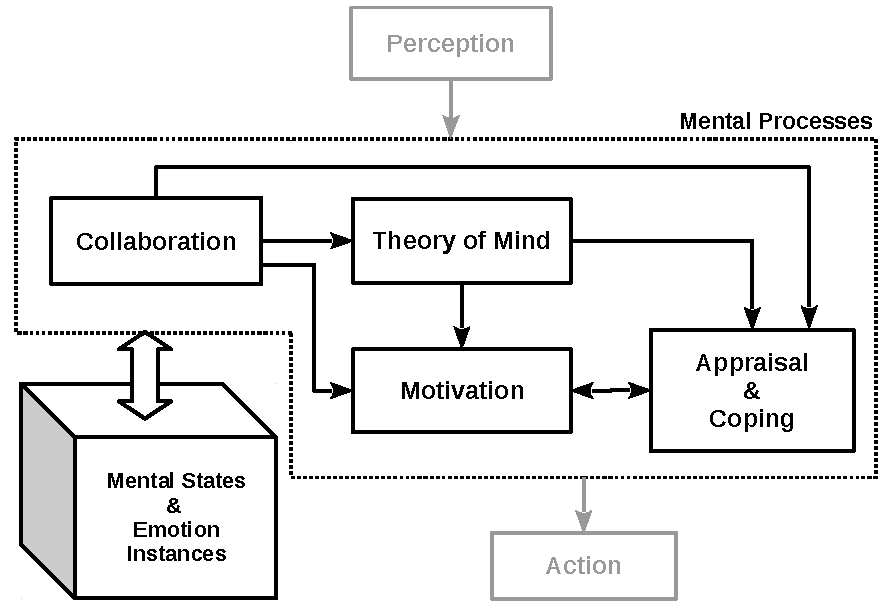
\includegraphics[scale=0.78]{figure/theory-general-croped.pdf}
  \caption{Computational framework based on \textit{Affective Motivational
  Collaboration Theory} (arrows indicate primary influences between
  mechanisms).}
  \label{fig:cpm}
\end{figure}

Affective Motivational Collaboration Theory focuses on the processes regulated
by emotional states. It aims to explain both rapid emotional reactions to events
as well as slower, more deliberative responses. These observable behaviors
represent the outcome of reactive and deliberative processes related to the
interpretation of the Robot's relationship to the collaborative environment.
These reactive and deliberative processes are triggered by two types of events:
\textit{external} events, such as the human's utterances and primitive actions,
and \textit{internal} events, comprising changes in the Robot's mental state,
such as belief formation and emotional changes. Affective Motivational
Collaboration Theory explains how emotions regulate the underlying processes in
the occurrence of these events during collaboration.

Emotion-regulated processes operate based on the Robot's mental state, which
also includes the anticipated mental state of the human, generated according to
the Robot's model of the human. These mental states include beliefs, intentions,
goals, motives and emotion instances. Each of these mental states possess
multiple attributes impacting the relation between cognition and behavior or
perception.

In summary, Affective Motivational Collaboration Theory consists of five
mechanisms all of which store and retrieve data in the Mental States. We will
describe each mechanism and their influences on each other briefly below.

\subsection{Collaboration Mechanism}
\label{sec:collaboration-mech}

The \textit{Collaboration} mechanism (see Fig.~\ref{fig:cpm}) constructs
a hierarchy of tasks and also manages and maintains the constraints and other
required details of the collaboration specified by the plan. These constraints
on task states and on the ordering of tasks include the inputs and outputs of
individual tasks, the preconditions specifying whether it is appropriate to
perform a task (which can be used as an indication of an impasse), and the
postconditions specifying whether a just-completed task was successful (or
failed). The Collaboration mechanism includes processes to update and monitor
the shared plan. It also keeps track of the focus of attention, which specifies
the salient objects, properties and relations at each point of the
collaboration. These processes depend on the operation of other mechanisms. For
instance, the Appraisal mechanism is required to evaluate the current mental
state with respect to the current status of the collaboration. Also, the
Appraisal and Motivation mechanisms provide interpretation of task failure and
the formation of a new mental state (e.g.\,an intention) respectively.

\subsection{Appraisal \& Coping Mechanisms}
\label{sec:appraisal-coping-mech}

Appraisal is a subjective evaluation mechanism based on individual processes
each of which computes the value of the appraisal variables. The Appraisal
mechanism is responsible for evaluating changes in the Robot's mental state, the
anticipated mental state of the human, and the state of the collaboration
environment. Collaboration requires the evaluative function of the Appraisal
mechanism for various reasons. The course of a collaboration is based on a full
or a partial plan \cite{grosz:collaboration,grosz:discourse-structure} which
needs to be updated as time passes and collaborators achieve, fail at or abandon
a task assigned to them. The failure of a task should not destroy the entire
collaboration. Appraising the environment and the current event helps the Robot
to update the collaboration plan in response to changes in the environment and
avoid further critical failures during collaboration. Appraisal also helps the
Robot to have a better understanding of the human's actions by making inferences
based on appraisal variables \cite{marsella:ema-process-model}
\cite{scherer:appraisal-processes}. Furthermore, in order to collaborate
successfully, a collaborator cannot simply use the plan and reach to the shared
goal; there should be an adaptation mechanism not only for updating the plan but
also the underlying mental state. The output of Appraisal can directly and
indirectly impact other mechanisms. For instance, the Motivation mechanism uses
this data to generate, compare and monitor motives based on the current internal
appraisal of the Robot as well as the appraisal of the environment.

The Coping mechanism is responsible for adopting the appropriate behavior
(action) with respect to interpretation of the ongoing internal and external
changes. The Coping mechanism provides the Robot with different coping
strategies associated with changes in the Robot's mental state with respect to
the state of the collaboration. In other words, the Coping mechanism produces
cognitive responses based on the appraisal patterns.

\subsection{Motivation Mechanism}
\label{sec:motivation-mech}

The \textit{Motivation} mechanism operates whenever the Robot a) requires a new
motive to overcome an internal impasse in an ongoing task, or b) wants to
provide an external motive to the human when the human faces a problem in a
task. In both cases, the Motivation mechanism uses the Appraisal mechanism to
compute attributes of the competing motives. The purpose of Motivation mechanism
in Affective Motivational Collaboration Theory is to generate new emotion-driven
goal-directed motives considered as ``potential'' intentions. These motives are
generated based on what the Robot believes about the environment including the
Robot and the other collaborator and the corresponding appraisals. The Robot
uses these motives to reach to a private or shared goal according to new
conditions caused by changes in the environment. The Motivation mechanism
consists of an arrangement of three distinct processes. First, several motives
are generated with respect to the current mental state. Only one of these
competing motives is most likely to become a new intention. Therefore, a
comparison process decides which motive is more likely to be consistent with the
current state based on the values of the motive attributes (e.g., motive
importance and motive urgency). Finally, the new motive will be used to form a
new intention. As a result, the Robot can take an action based on the new
intention to sustain the collaboration progress. Furthermore, the Motivation
mechanism can serve the Theory of Mind mechanism by helping the Robot to infer
the motive behind the human's current action.

\subsection{Theory of Mind Mechanism}
\label{sec:tom-mech}

The \textit{Theory of Mind} mechanism is the mechanism for inferring a model of
the human's anticipated mental state. The Robot uses the Theory of Mind
mechanism to infer and attribute beliefs, intentions, motives and goals to its
collaborator based on the user model it creates and maintains during
collaboration. The Robot progressively updates this model during the
collaboration. The refinement of this model helps the Robot to anticipate the
human's mental state more accurately, which ultimately impacts the quality of
the collaboration and the achievement of the shared goal. Furthermore, the Robot
can make inferences about the motive (or intention) behind the human's actions
using the Motivation mechanism. This inference helps the Robot to update its own
beliefs about the human's mental state. In the reverse appraisal process
\cite{gratch:reverse-appraisal}, the Robot also applies the Appraisal mechanism
together with updated beliefs about the human's Mental States to infer the
human's current mental state based on the human's emotional expression. Finally,
the Collaboration mechanism provides the collaboration structure, including
status of the shared plan with respect to the shared goal and the mutual beliefs
to the Theory of Mind mechanism. Consequently, any change to the Robot's model
of the human will update the Robot's mental state.

\subsection{Perception \& Action}
\label{sec:tom-mech}

Perception is outside of our theory and is responsible for producing the sensory
information used by the mechanisms in our framework; it is only a source of data
to the computational framework (see Fig.\,\ref{fig:cpm}). Thus, our
computational framework starts with high-level semantic representation of events
(including utterances). The output of the Perception component provides a
unified perception representation across all of the mechanisms.

The Action component in Fig.\,\ref{fig:cpm}, which is also outside of our
theory, functions whenever the Robot needs to show a proper behavior according
to the result of the internal processes of the collaboration procedure; it is
only a sink of data in our computational framework. The only input to the Action
component is provided by the Coping mechanism. This input will cause the Action
component to execute an appropriate behavior of the Robot. This input to Action
has the same level of abstraction as the output of the Perception mechanism,
i.e., it includes the Robot's utterances, primitive actions and emotional
expressions.

\subsection{Mental States \& Emotion Instances}
\label{sec:mental-states}

The Mental States shown in Fig.\,\ref{fig:cpm} comprise the knowledge base
required for all the mechanisms in the overall framework.

\subsubsection{Beliefs}
\label{sec:beliefs}

\textit{Beliefs} are a crucial part of the Mental States. We have two different
perspectives on categorization of beliefs. In one perspective, we categorize
beliefs based on whether or not they are shared between the collaborators. The
SharedPlans \cite{grosz:plans-discourse} theory is the foundation of this
categorization in which for any given proposition the Robot may have: a) private
beliefs (the Robot believes the human does not know these), b) the inferred
beliefs of the human (the Robot believes the human collaborator has these
beliefs), and c) mutual beliefs (the Robot believes both the Robot and the human
have these same beliefs and both of them believe that). From another
perspective, we categorize beliefs based on who or what they are about. In this
categorization, beliefs can be about the Robot, the human, or the environment.
Beliefs about the environment can be about internal events, such as outcomes of
a new appraisal or a new motive, or external events such as the human's offer,
question or request, and general beliefs about the environment in which the
Robot is situated. Beliefs can be created and updated by different processes.
They also affect how these processes function as time passes.

Beliefs have attributes and they impact different processes of the framework
such as the evaluation of an external event by the Appraisal mechanism, and
updates to the collaboration plan. We use three belief attributes in the Appraisal mechanism.
Belief \textit{strength} is about how strongly the self holds salient beliefs
about an object, an entity, or an anticipated behavior. The \textit{saliency} of
a belief is a cognitive attribute that pertains to how easily the self becomes
aware of a belief. The \textit{persistence} of a belief refers to how resistant
the belief is to changes.

\subsubsection{Intentions}
\label{sec:intentions}

\textit{Intentions} are mental constructs directed at future actions. They play
an essential role in: a) taking actions according to the collaboration plan, b)
coordination of actions with the human collaborator, c) formation of beliefs
about the Robot and anticipated beliefs about the human, and d) behavior
selection in the Coping mechanism. First, taking actions means that the Robot
will intend to take an action for primitive tasks that have gained the focus of
attention, possess active motives, and have satisfied preconditions for which
required temporal predecessors have been successfully achieved. Second,
intentions are involved in action coordinations in which the human's behavior
guides the Robot to infer an anticipated behavior of the human. Third,
intentions play a role in belief formation, mainly as a result of the permanence
and commitment inherent to intentions in subsequent processes, e.g., appraisal
of the human's reaction to the current action and self-regulation. Lastly,
intentions are involved in selecting intention-related strategies, e.g.,
planning, seeking instrumental support and procrastination, which is an
essential category of the strategies in the Coping mechanism
\cite{marsella:ema-process-model}. Intentions possess a set of attributes, e.g.
\textit{involvement, certainty, ambivalence} which moderate the consistency
between intention and behavior. The issue of consistency between the intentions
(in collaboration) and the behaviors (as a result of the Coping mechanism in the
appraisal cycle) is important because neither of these two mechanisms alone
provides solution for this concern.

\subsubsection{Motives}
\label{sec:motives}

\textit{Motives} are mental constructs which can initiate, direct and maintain
goal-directed behaviors. They are created by the emotion-regulated Motivation
mechanism. They are created by the emotion-regulated Motivation mechanism.
Motives can cause the formation of a new intention for the robot according to:
a) its own emotional states, b) its own private goal, c) the collaboration
(shared) goal, and d) other's anticipated beliefs. Motives possess a set of
attributes. The Motivation mechanism compares motives based on the quality of
these attributes and chooses the one which is the most related to the current
state of the collaboration. We use two motive attributes in Appraisal
mechanisms. The \textit{importance} of a motive is determined by the
corresponding beliefs about the effects of achieving or not achieving the
associated goal. The \textit{urgency} of a motive defines how much time the self
has to acknowledge and address that motive before it is too late. These
attributes are involved in the comparison of newly generated motives based on
the current state of the collaboration. Ultimately, the Robot forms or updates
an intention associated with the winning motive in the Mental States.

\subsubsection{Goals}
\label{sec:goals}

\textit{Goals} help the Robot to create and update the structure of the
collaboration plan. Goals direct the formation of intentions to take appropriate
corresponding actions during collaboration. Goals also drive the Motivation
mechanism to generate required motive(s) in uncertain or ambiguous situations,
e.g., to minimize the risk of impasse or to reprioritize goals. Goals have
three attributes. The \textit{specificity} of goals has two functions for the
Robot. First, it defines the performance standard for evaluating the progress
and quality of the collaboration. Second, it serves the Robot to infer the
winner of competing motives. The \textit{proximity} of goals distinguishes goals
according to how ``far'' they are from the ongoing task. Proximal (or
short-term) goals are achievable more quickly, and result in higher motivation
and better self-regulation than more temporally distant (or long-term) goals.
Goals can influence the \textit{strength} of beliefs, which is an important
attribute for regulating the elicitation of social emotions. The
\textit{Difficulty} of goals impacts collaborative events and decisions in the
appraisal, reverse appraisal, motive generation and intention formation
processes. For instance, overly easy goals do not motivate; neither are humans
motivated to attempt what they believe are impossible goals.

\subsubsection{Emotion Instances}

\textit{Emotions} in Mental States are emotion instances that are elicited by
the Appraisal mechanism. These emotion instances include the Robot's own
emotions as well as the anticipated emotions of the human which are created with
the help of the processes in the Theory of Mind mechanism, e.g., worry.

\section{Collaboration}

The Collaboration mechanism constructs a hierarchy of goals associated with
tasks in the form of a hierarchical task network (see Figure \ref{fig:cs}), and
also manages and maintains the constraints and other required details of the
collaboration including the inputs and outputs of individual tasks, the
\textit{preconditions} (specifying whether it is appropriate to perform a task),
and the \textit{postconditions} (specifying whether a just-completed task was
successful). Collaboration also keeps track of the focus of attention, which
determines the salient objects, properties and relations at each point, and
shifts the focus of attention during the interaction.

\begin{figure}[tbh]
  \centering
  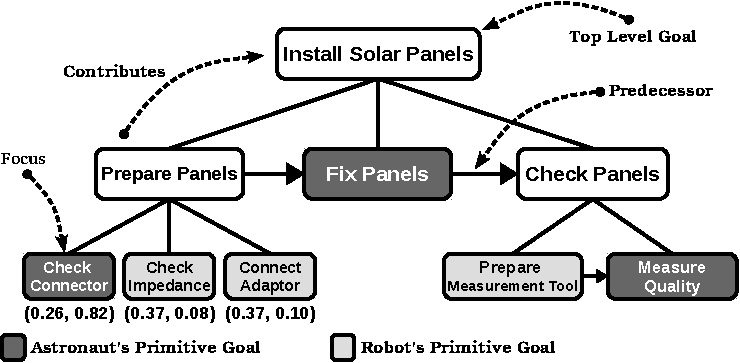
\includegraphics[width=\textwidth]{figure/collaborationStructure-croped.pdf}
  \caption{{\fontsize{9}{9}\selectfont Collaboration structure (shared plan).}}
  \label{fig:cs}
\end{figure}

Here, we briefly describe the methods which retrieve information about the
collaboration structure, and are used in our algorithms to compute the values of
appraisal variables. In these methods, $\varepsilon_t$ is the event
corresponding to time \textit{t}, and $g_t$ is a given goal at time \textit{t}.

\begin{itemize}[leftmargin=2pt]
  \setlength\itemsep{1mm}
  \item \textit{recognizeGoal($\varepsilon_t$)} returns the unique goal to which
  the given event (action, utterance, or emotional expression) directly
  contributes; it is only one goal since the robot can only do one primitive
  action at a time in our collaboration model, i.e, in the goal tree, a given
  primitive action can only directly contribute to one parent goal. The method
  returns \textit{ambiguous} if it does not recognize a goal in the
  plan\footnote{Ambiguity introduces some extra complexities which are beyond
  scope of this paper.}.
  
  \item \textit{getGoalStatus($g_t$)} returns whether $g_t$'s status is
  \textsc{achieved, failed, blocked, inapplicable, pending,} or \textsc{in
  progress}. In our example, ``Check Connector'' is the current (focused) goal
  and it is \textsc{pending}, and the ``Prepare Panels'' and ``Install Solar
  Panels'' are \textsc{in progress}. The focused goal is the goal that the robot
  currently pursues.
  
  \item \textit{getTopLevelGoal($g_t$)} returns $g_t$'s top level goal.
  
  \item \textit{currGoalStatus($g_t$)} returns the current goal status whether
  it is \textsc{achieved, failed, blocked, inapplicable, pending,} or \textsc{in
  progress}. In our example, ``Prepare Measurement Tool'' is the current
  (focused) goal.

  \item \textit{precondStatus($g_t$)} returns the status of the precondition for
  the given goal whether it is \textsc{satisfied, unsatisfied} or
  \textsc{unknown}. For instance, the precondition for fixing a panel is whether
  the panel is appropriately located on its frame.
  
  \item \textit{isLive($g_t$)} returns \textit{true} if all the predecessors of
  $g_t$ are \textsc{achieved} and all the preconditions are \textsc{satisfied},
  i.e., \textsc{pending} or \textsc{in progress} goals; otherwise returns
  \textit{false}.
  
  \item \textit{isFocusShift($g_t$)} returns \textit{true} if the given
  goal is not the previous focus (top of the stack); otherwise returns
  \textit{false}.
  
  \item \textit{isNecessaryFocusShift($g_t$)} returns \textit{true} if the
  status of the previous focus was \textsc{achieved}; otherwise returns
  \textit{false} \cite{rich:focused-unfocused-users}.
  
  \item \textit{isPath($g_1$, $g_2$)} returns \textit{true} if there is a path
  between $g_1$ and $g_2$ in a plan tree structure; otherwise returns
  \textit{false}.
  
%   \item \textit{doesContribute($g_t$)} returns whether the given goal
%   contributes to another goal in the higher level of the plan hierarchy. For
%   instance, an abstract (nonprimitive) goal of ``Bring Panels'' contributes to
%   the higher level goal of ``Install Solar Panels''.
  
  \item \textit{getContributingGoals($g_t$)} returns $g_t$'s children.
  
  \item \textit{getPredecessors($g_t$)} returns $g_t$'s predecessors.
  
  \item \textit{getInputs($g_t$)} returns all required inputs for $g_t$. For
  example, the goal ``Fix Panels'' requires inputs such as \textit{welding tool}
  and \textit{panel}.
  
  \item \textit{isAvailable($g_t$)} returns whether the given input is
  available. For instance, whether the \textit{welding tool} is available for the
  goal ``Fix Panels''.
  
%   \item \textit{isAchieved($g_t$)} returns whether the given goal is achieved,
%   i.e., whether all the postconditions of the given goal are \textsc{satisfied}.
  
  \item \textit{isFocused($g_t$)} returns whether the focus is on $g_t$.
  
  \item \textit{getResponsible($g_t$)} returns responsible agent(s) for $g_t$.
  In a dyadic collaboration, both of the agents (joint) can be partly responsible
  for a nonprimitive goal, while each (self or other) is responsible for one or
  more primitive goals. For instance, both the robot and the astronaut are
  responsible for the nonprimitive goal of ``Install Solar Panels'', whereas it
  is only the astronaut who is responsible for the primitive goal of ``Prepare
  Measurement Tool''.
\end{itemize}

\section{Appraisal Processes}
\label{sec:appraisal}

We consider four appraisal variables to be the most important appraisal
variables in a collaboration context, i.e., \textit{Relevance} (since other
appraisals are only computed for relevant events), \textit{Desirability}
(Algorithm \ref{alg:desirability}), \textit{Expectedness} (Algorithm
\ref{alg:expectedness}), and \textit{Controllability} (since it is associated
with the agent's coping ability). There are other appraisal variables introduced
in psychological \cite{scherer:appraisal-processes} and computational literature
\cite{gratch:domain-independent}. We believe most of these variables can be
straightforwardly added to our appraisal mechanism later. All of the algorithms
in this section use mental states of the robot (discussed in Section
\ref{sec:mental-states}) which are formed based on the collaboration structure.
These algorithms use the corresponding recognized goal of the most recent event
at each turn.

\subsection{Relevance}

Relevance is an important appraisal variable since the other appraisal variables
are meaningful only for relevant events. Relevance as an appraisal variable
measures the significance of an event for the self. An event can be evaluated to
be relevant if it has a non-zero utility \cite{marsella:ema-process-model}.
However, the utility of an event is also influenced by the other collaborator's
emotional expressions as the reflection of the other collaborator's mental state
with respect to the status of the collaborative environment. Other appraisal
models only consider the utility of an event based on the self's (robot's) goal
and plan.

Algorithm \ref{alg:relevance} determines the relevance of the given event with
respect to the current mental state. The relevance of the event depends on the
significance of the event with respect to the collaboration status, which is
determined based on the utility of the event as presented in
\cite{gratch:domain-independent,marsella:ema-process-model}. Our algorithm for
computing the relevance of an event during collaboration involves other factors
that other appraisal models do not consider. For instance, the human's
perceived emotion, recurrence of a belief, or occurrence of a belief about an
unrelated goal by the human play important roles by influencing the utility
of an event during collaboration. As a result, evaluating the relevance of
events can cause a collaborative robot to respond effectively which can
positively impact the status of the shared goal, without dedicating all its
resources to every event.

After perceiving an event, the belief about that event represents the event in
the robot's mental state. \textit{recognizeGoal} returns the goal to which the
current event contributes, unless it is \textit{ambiguous}\footnote{Ambiguity
introduces some extra complexities which are beyond scope of this paper.};
$g_{t}$ represents the shared goal at time (turn) $t$ within the shared plan. We
compute the utility ($-1 \leq \mathcal{U} \leq 1$) of the event using the values
of the attributes associated with the existing beliefs, and the attributes of
the motive associated with the recognized goal (see details below). We use three
belief attributes (see Section \ref{sec:mental-states}) to compute the
belief-related part of the utility:

\begin{algorithm}
	\caption{(Relevance)}
	\label{alg:relevance}
	\begin{algorithmic}[1]
		\Function{IsEventRelevant}{Event $\varepsilon_t$}
			\Statex
			\State $\mathit{g}_{t} \gets \textit{recognizeGoal}{(\varepsilon_t)}$
			\Statex
			\State $\mathcal{U} \gets \Call{getEventUtility}{\mathit{g}_{t}}$ 
			\State $\tau_{t} \gets \Call{getEmotionalThreshold}{\mathit{g}_{t}}$
			\Statex
			\If {$( \mathcal{U} \geq \tau_{t} )$}
				\State \Return {{\fontsize{7}{8}\selectfont RELEVANT}}
			\Else
				\State \Return {{\fontsize{7}{8}\selectfont IRRELEVANT}}
			\EndIf
		\EndFunction
	\end{algorithmic}
\end{algorithm}

\begin{itemize}[leftmargin=2pt]
  \setlength\itemsep{0.2mm}
  \item \textit{Strength}: The extent to which the preconditions ($\alpha$),
  postconditions ($\beta$), predecessors ($\lambda$), and contributing goals
  ($\mu$) of a goal are known (\textsc{satisfied} or \textsc{unsatisfied}) makes
  beliefs about the goal stronger. An \textsc{unknown} pre and postcondition
  status of a goal and its predecessors and contributing goals forms weaker
  beliefs. For instance, if one knows all predecessors of a pursued goal (e.g.,
  ``Press Bread Slices'') are \textsc{satisfied} (i.e., ``Spread Peanut Butter''
  and ``Spread Strawberry Jam''), failure of the pursued goal will elicit one's
  negative emotion (due to the strong beliefs related to the goal); whereas not
  knowing the status of the goal-related factors (e.g., whether Mary could find
  the knife to cut the sandwich in half) causes one to form weaker beliefs about
  the goal.
  \item \textit{Saliency (S)}: Beliefs related to the focused goal are more
  salient than beliefs related to any other goal in the plan; according to
  Figure \ref{fig:taskModel}, if one is making a boiled egg sandwich, beliefs
  related to all of the other \textit{live} (\textsc{pending} or \textsc{in
  progress}) goals (e.g. ``Pack Sandwich'') will be less salient than beliefs
  related to the focused goal, i.e., ``Add Pickles''. Beliefs' saliency
  decreases according to their corresponding \textit{live} goal's distance from
  the focused goal in the shared plan. \textit{Non-live} goals will not be
  salient.
  \item \textit{Persistence (P)}: The recurrence of a belief over time (turns)
  increases the persistence of the belief. Beliefs occurring only once have the
  lowest value of persistence. For instance, if Mary keeps saying that she can
  not find the knife to cut the sandwich in half, one could pursue a new goal
  outside of the shared plan to acknowledge Mary's concern.
\end{itemize}

\noindent We also use two motive attributes discussed in Section
\ref{sec:mental-states} to compute the motive related part of the utility
($\mathcal{U}$):

\begin{itemize}[leftmargin=2pt]
  \setlength\itemsep{0.05mm}
  \item \textit{Urgency ($\gamma$)}: There are two factors impacting the urgency
  of a motive: a) whether the goal directing the given motive is the predecessor of
  another goal for which the other collaborator is responsible, and b) whether
  achieving the goal directing the given motive can mitigate the other
  collaborator's negative valenced emotion. For instance, if one has a private
  goal to prepare for making the second sandwich (e.g. get the eggs) while Mary
  is waiting to get the first sandwich and cut it in half, pressing bread slices
  and passing them to Mary will be more urgent than one's private goal.
  \item \textit{Importance ($\eta$)}: A motive is important if failure of the
  directing goal causes an impasse in the shared plan (i.e., no further goal is
  available to achieve), or achievement of the directing goal removes an
  existing impasse. For example, if one cannot find white bread on which to
  spread peanut butter (an impasse to make the peanut butter sandwich), and Mary
  offers to use wheat bread instead (external motive), the new motive becomes
  important to remove the impasse in the shared plan.
\end{itemize}

We provide the utility function ($\mathcal{U}$) in Equation \ref{eqn:utility}.
This function uses: saliency (\textit{S}) and persistence (\textit{P}) of the
belief related to the recognized goal, the recognized goal's status
($\upsilon$), and the aggregation of belief and motive attributes ($\Psi$)
according to Equation \ref{eqn:power}.

\begin{equation}
    \mathcal{U}(\varepsilon_t)= 
    \begin{dcases}
       \upsilon\!P\cdot S^{\Psi} & \Psi \textgreater 0 \\
       0               			 & \Psi = 0
    \end{dcases}
    \label{eqn:utility}
\end{equation}

Intuitively, we use $\upsilon$ to generate positive and negative utility values.
The $\upsilon$'s value becomes +1 if the status of the corresponding goal is
\textsc{achieved}, \textsc{pending}, or \textsc{in progress}, and $\upsilon$'s
value becomes -1 if the status of the corresponding goal is \textsc{failed,
blocked}, or \textsc{inapplicable}. The \textit{P} influences the value of
utility only as a coefficient since recurrent beliefs are not formed frequently
during collaboration. The $\Psi$ value indicates the magnitude of the influence
of beliefs and motives using their attributes. Hence, the $\Psi$ value impacts
the saliency value of beliefs exponentially, helping to differentiate between
beliefs.

In equation \ref{eqn:power}, the subscript \textit{k} refers to the
\textit{known} goal-related factors (\textsc{satisfied} or
\textsc{unsatisfied}); whereas the subscript \textit{all} includes both
\textit{known} and \textit{unknown} goal-related factors. In this equation, both
urgency ($\gamma$) and importance ($\eta$) attributes of motives can impact the
outcome of the goal-related belief attributes' ratio, and ultimately the $\Psi$
value.

\begin{equation}
    \Psi = \frac{\alpha_{_k} + \beta_{_k} + \lambda_{_k} +
    \mu_{_k}}{\alpha_{_{all}} + \beta_{_{all}} + \lambda_{_{all}} +
    \mu_{_{all}}} + \eta + \gamma
    \label{eqn:power}
\end{equation}

\begin{center} 
    $\eta, \gamma \in \mathbb{N}, \qquad\qquad \eta, \gamma \geq 0$\\
    $\alpha_{_k}, \beta_{_k}, \lambda_{_k}, \mu_{_k} \in \mathbb{N},
    \qquad\qquad \alpha_{_k}, \beta_{_k}, \lambda_{_k}, \mu_{_k} \geq 0$\\
    $\alpha_{_{all}}, \lambda_{_{all}}, \mu_{_{all}} \in \mathbb{N},
    \qquad\qquad \alpha_{_{all}}, \lambda_{_{all}}, \mu_{_{all}} \geq 0$\\
    $\beta_{_{all}} \in \mathbb{N}, \qquad\qquad \beta_{_{all}} \geq 1$
\end{center}

The significance of an event in a collaborative environment is based on the
utility of the event and the human's perceived emotion. The human's perceived
emotion influences the relevance of the event in the form of a threshold value
$\tau_{t}$. In Equation \ref{eqn:threshold}, we use the valence of the perceived
emotion ($\mathcal{V}_{e_h}$) to compute $\tau_{t}$.

\begin{equation}
    \tau_{t}= 
    \begin{dcases}
       1-\mathcal{V}_{e_h} & \mathcal{V}_{e_h} > 0 \\
       |\mathcal{V}_{e_h}| & \mathcal{V}_{e_h} \leq  0
    \end{dcases}
    \label{eqn:threshold}
\end{equation}

\begin{center} 
    $\mathcal{V}_{e_h} \in \mathbb{R}, \qquad\qquad -1 \leq \mathcal{V}_{e_h}
    \leq 1$
\end{center}

Hence, perceiving human's positive emotion (e.g., happiness) reduces the
threshold value which makes the robot find an event \textsc{relevant} with even
a slightly positive utility. Similarly, an event can be considered
\textsc{irrelevant} even though the utility has a relatively positive value,
because of perceiving the human's negative emotion.

\subsection{Desirability}

Desirability characterizes the value of an event to the robot in terms of
whether the event facilitates or thwarts the collaboration goal. Desirability
captures the valence of an event with respect to the robot's preferences
\cite{gratch:domain-independent}. In a collaborative robot, preferences are
biased towards those events facilitating progress in the collaboration.
Desirability plays an important role in the overall architecture; it makes the
processes involved in the other mechanisms (e.g., Motivation and Theory of
Mind) and consequently the robot's mental state, congruent with the
collaboration status which is a collaborative robot's desire. Therefore, it
causes the robot to dismiss events causing inconsistencies in the robot's
collaborative behavior. Moreover, desirability is also crucial from the
collaboration's point of view.

% A collaborative robot needs to know whether its own and the other collaborator's
% actions, utterances, and emotional expressions are desirable in terms of their
% consistence with the status of the current shared goal. In other words, the
% collaboration mechanism uses the appraisal process of desirability to coordinate
% what the self or the other does, says, and expresses during collaboration.
% Reciprocally, the appraisal mechanism and in this case the desirability process
% use the collaboration structure to obtain their required information.

\begin{algorithm}[tbh]
	\caption{(Desirability)}
	\label{alg:desirability}
	\begin{algorithmic}[1]
		\Function{IsEventDesirable}{Event $\varepsilon_t$}
			\Statex
			\State $\mathit{g}_{t} \gets \textit{recognizeGoal}{(\varepsilon_t)}$
			\State $\mathit{g}_{top} \gets \textit{getTopLevelGoal}{(\mathit{g}_{t})}$
			\Statex
			\If {$(\mathit{g}_{t} =$ {\fontsize{8}{9}\selectfont AMBIGUOUS}$)$} 
				\State \Return {\fontsize{8}{9}\selectfont UNDESIRABLE}
			\EndIf
			\Statex
			\If {(\textit{getGoalStatus($g_{top}$)} =
			{\fontsize{8}{9}\selectfont ACHIEVED})}
			\State \Return {{\fontsize{8}{9}\selectfont MOST-DESIRABLE}} 
			\ElsIf {(\textit{getGoalStatus($g_{top}$)} =
			{\fontsize{8}{9}\selectfont FAILED})} 
			\State \Return {{\fontsize{8}{9}\selectfont MOST-UNDESIRABLE}}
			\ElsIf {(\textit{getGoalStatus($g_{top}$)} =
			{\fontsize{8}{9}\selectfont BLOCKED}) \OR\\
			\hspace*{5mm}(\textit{getGoalStatus($g_{top}$)} =
			{\fontsize{8}{9}\selectfont INAPPLICABLE})}
			\State \Return {{\fontsize{8}{9}\selectfont UNDESIRABLE}} 
			\ElsIf {(\textit{getGoalStatus($g_{top}$)} =
			{\fontsize{8}{9}\selectfont PENDING}) \OR\\
			\hspace*{5mm}(\textit{getGoalStatus($g_{top}$)} =
			{\fontsize{8}{9}\selectfont INPROGRESS})}
				\Statex
				\If {(\textit{getGoalStatus($g_{t}$)} =
				{\fontsize{8}{9}\selectfont ACHIEVED})}
				\State \Return {{\fontsize{8}{9}\selectfont DESIRABLE}}
				\ElsIf {(\textit{getGoalStatus($g_{t}$)} = {\fontsize{8}{9}\selectfont
				FAILED})} 
				\State \Return {{\fontsize{8}{9}\selectfont MOST-UNDESIRABLE}}
				\ElsIf {(\textit{getGoalStatus($g_{t}$)} = {\fontsize{8}{9}\selectfont
				BLOCKED}) \OR \\
				\hspace*{10mm}(\textit{getGoalStatus($g_{t}$)} =
				{\fontsize{8}{9}\selectfont INAPPLICABLE})} 
				\State \Return {{\fontsize{8}{9}\selectfont UNDESIRABLE}}
				\ElsIf {(\textit{getGoalStatus($g_{t}$)} =
				{\fontsize{8}{9}\selectfont PENDING}) \OR \\ \hspace{1mm} 
				\hspace*{8mm}(\textit{getGoalStatus($g_{t}$)} =
				{\fontsize{8}{9}\selectfont INPROGRESS})} 
				\State \Return {{\fontsize{8}{9}\selectfont NEUTRAL}}
				\EndIf
			\EndIf
		\EndFunction
	\end{algorithmic}
\end{algorithm}

Algorithm \ref{alg:desirability} provides a process in which the desirability of
an event is computed with regard to the status of the shared goal; i.e., it
operates based on whether and how the event changes the status of the current
shared goal. It distinguishes between the top level goal and the current goal
because the top level goal's change of status attains a higher positive or
negative value of desirability. For instance, failure of the top level goal
(e.g., installing solar panel) is more undesirable than failure of a primitive
goal (e.g., measuring the quality of the installed panel).

An \textsc{ambiguous} goal is a goal associated with the current event
($\varepsilon_t$) which is not recognized in the robot's plan; therefore it is
\textsc{undesirable} for a collaborative robot. A top level goal' status must be
\textsc{achieved} (i.e., \textsc{satisfied} postcondition) to consider the event
\textsc{most-desirable}. When the goal's status is \textsc{failed} (i.e.,
\textsc{unsatisfied} postcondition) or \textsc{blocked}, the associated event
has the \textsc{most-undesirable} or \textsc{undesirable} values respectively.
A goal is \textsc{blocked} if any of the required goals or goals recursively
through the parent goal are not \textsc{achieved}. An \textsc{inapplicable} goal
is also considered as \textsc{undesirable}. A goal is \textsc{inapplicable} if
any of its predecessors are not \textsc{achieved}, and/or its preconditions are
not \textsc{satisfied}. For \textsc{pending} and \textsc{inprogress} top level
goals, the status of the current goal associated with the top level goal
determines the status of the event $\varepsilon_t$. Only a non-primitive goal
can have \textsc{inprogress} status, if it has been started but is not yet
completed. A goal can be \textsc{pending} if it is live, or if it is a
non-primitive goal that has not been started yet. \textsc{Achieved} current
goals mark an event ($\varepsilon_t$) as \textsc{desirable}, while
\textsc{failed} or \textsc{blocked} current goals render the event associated
with them as \textsc{most-undesirable} and \textsc{undesirable} respectively.
\textsc{Pending} or \textsc{inprogress} current goals mark their associated
events as \textsc{neutral}.

\vspace*{-2mm}
\subsection{Expectedness}

Expectedness is the extent to which the truth value of a state could have been
predicted from causal interpretation of an event. In the collaboration context
the expectedness of an event evaluates the congruency of the event with respect
to the existing knowledge about the shared goal. Thus, expectedness underlies a
collaborative robot's attention. The collaboration mechanism uses expectedness
to maintain the robot's attention and subsequently its mental state with respect
to the shared goal. Reciprocally, the appraisal mechanism uses the underlying
information of the collaboration structure to evaluate the expectedness of an
event \cite{shayganfar:appraisal-short}.

\begin{algorithm}[t]
	\caption{(Expectedness)}
	\label{alg:expectedness}
	\begin{algorithmic}[1]
		\Function{IsEventExpected}{Event $\varepsilon_t$}
			\Statex
			\State $\mathit{g}_{t} \gets \textit{recognizeGoal}{(\varepsilon_t)}$
			\State $\mathit{g}_{top} \gets \textit{getTopLevelGoal}{(\mathit{g}_{t})}$
			\Statex
			\If {$(\textit{isLive}{(\mathit{g}_{t})})$}
				\If {$(\neg \textit{isFocusShift}{(\mathit{g}_{t})}\hspace*{2mm}\OR$ \\
				\hspace*{13mm}$\textit{isNeccessaryFocusShift}{(\mathit{g}_{t})})$}
				\State \Return {\fontsize{7}{8}\selectfont MOST-EXPECTED}
				\Else
					\State \Return {\fontsize{7}{8}\selectfont EXPECTED}
				\EndIf
			\Else
				\If {$(\textit{isPath}{(\mathit{g}_{t}, \mathit{g}_{top})})$}
					\State \Return {\fontsize{7}{8}\selectfont UNEXPECTED}
				\Else
					\State \Return {\fontsize{7}{8}\selectfont MOST-UNEXPECTED}
				\EndIf
			\EndIf
		\EndFunction
	\end{algorithmic}
\end{algorithm}

In Algorithm \ref{alg:expectedness} we provide the process of computing the
expectedness based on the shared plan and status of the shared goal. The key
point in this algorithm is the status of the current shared goal
($\mathit{g}_{t}$), which is associated with the event $\varepsilon_t$ and its
relationship with the top level goal ($\mathit{g}_{_{top}}$).

The intuition captured here is that one expects the current goal to be finished
before undertaking another activity, but the goals that can be the next focus of
attention are also to be expected. Therefore, if the goal is live, the algorithm
checks whether the goal has not changed, or whether the interpretation of the
last event results in a necessary focus shift. Shifting the focus to a new goal
is necessary when the former goal is achieved and a new goal is required.
Consequently the new event is the \textsc{most-expected} one. However, even if
the focus shift is not necessary, the new event can be considered as
\textsc{expected}, since the corresponding goal is already live. For goals that
have not yet been started (that is, are not live), the algorithm must determine
how unexpected it would be to pursue one now; if the goal is at least in the
plan, i.e., on the path to the top level goal, it is just \textsc{unexpected}
while any others are \textsc{most-unexpected}.

\subsection{Controllability}
\label{sec:controllability}

Controllability is the extent to which an event can be influenced; it is
associated with a robot's ability to cope with an event
\cite{gratch:domain-independent}. Thus, a robot can determine whether an event's
outcome can be altered by actions under either of the collaborators' control. In
other words, controllability is a measure of a robot's ability to maintain or
change a particular state as a consequence of an event.

\begin{algorithm}
	\caption{(Controllability)}
	\label{alg:controllability}
	\begin{algorithmic}[1]
		\Function{IsEventControllable}{Event $\varepsilon_t$}
 			\State $\mathit{g}_{t} \gets \textit{recognizeGoal}{(\varepsilon_t)}$
  			\Statex
			\State $\mathcal{M} \gets \Call{GetAgencyRatio}{\mathit{g}_{t}}$ 
			\State $\mathcal{R} \gets \Call{GetAutonomyRatio}{\mathit{g}_{t}}$
 			\Statex
			\State $\mathcal{P} \gets \Call{GetSuccPredecessorsRatio}{\mathit{g}_{t}}$
			\State $\mathcal{I} \gets \Call{GetAvailableInputs}{\mathit{g}_{t}}$
  			\Statex
			\State $\mathcal{V}_{e_h} \gets \Call{getEmotionValence}{\mathit{g}_{t}}$ 
			\State $\omega \gets \Call{getWeights}{\mathit{g}_{t}}$
			\Statex
			\State $\mathcal{X} \gets
			\frac{\omega_{0}\cdot \mathcal{M} + \omega_{1}\cdot \mathcal{R} +
			\omega_{2}\cdot \mathcal{P} + \omega_{3}\cdot \mathcal{I}}{\omega_{0} +
			\omega_{1} + \omega_{2} + \omega_{3}} + \mathcal{V}_{e_h}$
  			\Statex
% 			\State $\tau_{t} \gets \Call{getEmotionalThreshold}{\mathit{g}_{t}}$
 			\Statex
			\If {$(\mathcal{X} > 0)$}
 				\State \Return {{\fontsize{7}{8}\selectfont CONTROLLABLE}}
			\Else
 				\State \Return {{\fontsize{7}{8}\selectfont UNCONTROLLABLE}}
			\EndIf
		\EndFunction
	\end{algorithmic}
\end{algorithm}

Controllability is important for the overall architecture. For instance, the
robot can choose to ask or negotiate about a collaborative task which is not
controllable, or form a new motive to establish an alternative goal for the
current uncontrollable event. In general, other mechanisms in the architecture
use the controllability output in their decision making processes; meanwhile
controllability uses information from the collaboration structure, e.g.,
predecessors of a goal.

An important determinant of one's emotional response is the sense of control
over occurring events. This sense of subjective control is based on one's
reasoning about self's power. For instance, the robustness of one's plan for
executing actions can increase one's sense of power and subsequently the sense
of control. In the collaboration context, we have translated the sense of control
into a combination of four different factors including a) \textit{agency} and b)
\textit{autonomy} of the robot, as well as the ratios of c) \textit{successful
predecessors}, and d) the \textit{available inputs} of a given goal
(i.e., $\mathit{g}_{t}$) in the shared plan.

In Algorithm \ref{alg:controllability}, we partially compute the controllability
of an event based on the above four factors. We use weighted averaging of these
factors to determine their impact on the controllability of an event (line 9).
The value of all these weights are set to \textit{1.0} for the purpose of
simplicity at this stage (\textbf{$\Call{getWeights}{}$}). We will adjust these
weights after further investigating the influence of these factors, and
implementing other mechanisms in the overall architecture. We believe that the
human's perceived emotion also impacts the controllability of an event
(\textbf{$\Call{getEmotionValence}{}$}). The ($-1.0 \leq \mathcal{V}_{e_h} \leq
1.0$) is the valence value of the human's perceived emotion. Positive emotions,
e.g., happiness, possess positive values, and negative emotions, e.g., anger,
have negative values. The magnitude of this value can change with respect to the
intensity of the perceived emotion. Thus, a positive controllability value
indicates that an event is \textsc{controllable}; otherwise
\textsc{uncontrollable}.

% \renewcommand\thealgorithm{4\alph{algorithm}}
% \setcounter{algorithm}{0}
% 
% \begin{algorithm}
% 	\caption{(Get Agency Ratio)}
% 	\label{alg:agency}
% 	\begin{algorithmic}[1]
% 		\Function{GetAgencyRatio}{Event $\varepsilon_t$}
% 			\Statex
% 			\State $\mathit{g}_{t} \gets \textit{recognizeGoal}{(\varepsilon_t)}$
% 			\Statex
% 			\State $\mathcal{M}_{t} \gets \textit{getActiveMotive}{(\mathit{g}_{t})}$
% 			\Statex
% 			\If {$(\mathcal{M}_{t} \neq \emptyset)$}
% 				\If {$(\mathcal{M}_{t}\cdot type = $
% 				{{\fontsize{8}{8}\selectfont INTERNAL}}$)$} \State \Return {1.0}
% 				\Else
% 					\State \Return {0.0}
% 				\EndIf
% 			\Else
% 				\State \Return {0.0}
% 			\EndIf
% 		\EndFunction 
% 	\end{algorithmic}
% \end{algorithm}

$\Call{\textbf{GetAgencyRatio}}{}$: \textit{Agency} is the capacity of an
individual to act independently in a given environment. In a collaborative
environment collaborators are sometimes required to act independently of each
other. Hence, they need to have some internal motives that are formed based on
their own mental states rather than motives that are reinforced by the other.
These internal motives will lead the collaborators to acquire new intentions
when required. If the robot's mental state possesses only an internal motive
supporting the recognized goal, we consider a maximum agency value denoted as
$\mathcal{M}$ in Algorithm \ref{alg:controllability} (i.e., $\mathcal{M}=1.0$);
otherwise we consider the minimum agency value (i.e., $\mathcal{M}=0.0$). Note
that the process of forming new internal motives is beyond scope of this paper.

% \renewcommand\thealgorithm{4\alph{algorithm}}
% \setcounter{algorithm}{1}
% 
% \begin{algorithm}
% 	\caption{(Get Autonomy Ratio)}
% 	\label{alg:autonomy}
% 	\begin{algorithmic}[1]
% 		\Function{GetAutonomyRatio}{Event $\varepsilon_t$}
% 			\Statex
% 			\State $\mathit{g}_{t} \gets \textit{recognizeGoal}{(\varepsilon_t)}$
% 			\Statex
% 			\State $\Phi_{\mathit{g}} \gets
% 			\textit{extractContributingGoals}{(\mathit{g}_{t})}$
% 			\Statex
% 			\ForAll {$\phi_{\mathit{g}}^i \in \Phi_{\mathit{g}}$}
% 				\If {$(\textit{getResponsible}{(\phi_{\mathit{g}}^i)} =$
% 				{\fontsize{8}{8}\selectfont SELF})} 
% 					\State $count_{self} \gets count_{self} + 1$
% 				\EndIf
% 			\EndFor
% 			\Statex
% 			\State \Return 
% 			${count_{self} \mathbin{/} {{\Phi_{\mathit{g}}}.total()}}$
% 		\EndFunction 
% 	\end{algorithmic}
% \end{algorithm}

$\Call{\textbf{GetAutonomyRatio}}{}$: \textit{Autonomy} is the ability to make
decisions without the influence of others, and implies acting on one's own and
being responsible for that. In a collaborative environment, tasks are delegated
to the collaborators based on their capabilities. Therefore, each collaborator
is responsible for the delegated task and the corresponding goal. In Algorithm
\ref{alg:controllability}, $\mathcal{R}$ denotes the value of autonomy with
regard to the goal $\mathit{g}_{t}$. This value $(0.0 \leq \mathcal{R} \leq
1.0)$ is the ratio of the number of goals contributing to $\mathit{g}_{t}$ for
which the robot is responsible over the total number of contributing goals, if
the goal associated with the current event is a nonprimitive goal. However, if
the associated goal of the current event corresponds to a primitive goal the
value of $\mathcal{M}$ would be 0.0 or 1.0. In general, higher autonomy leads to
a more positive value of controllability.

% \renewcommand\thealgorithm{4\alph{algorithm}}
% \setcounter{algorithm}{2}
% 
% \begin{algorithm}
% 	\caption{(Get Successful Predecessors Ratio)}
% 	\label{alg:predecessors}
% 	\begin{algorithmic}[1]
% 		\Function{GetSucPredecessorsRatio}{Event $\varepsilon_t$}
% 			\Statex
% 			\State $\mathit{g}_{t} \gets \textit{recognizeGoal}{(\varepsilon_t)}$
% 			\Statex
% 			\State $\Theta{\mathit{g}} \gets
% 			\textit{extractPredecessors}{(\mathit{g}_{t})}$
% 			\Statex
% 			\ForAll {$\theta_{\mathit{g}}^i \in \Theta_{\mathit{g}}$}
% 				\If {$(\textit{isAchieved}{(\theta_{\mathit{g}}^i)})$}
% 					\State $count_{achieved} \gets count_{achieved} + 1$
% 				\EndIf
% 			\EndFor
% 			\Statex
% 			\State \Return
% 			${count_{achieved} \mathbin{/} {\Theta{\mathit{g}}.total()}}$
% 		\EndFunction 
% 	\end{algorithmic}
% \end{algorithm}

$\Call{\textbf{GetSuccPredecessorsRatio}}{}$: The structure of a shared plan
contains the order of the required \textit{predecessors} of a goal. Predecessors
of a goal, $g_t$, are goals that the collaborators should achieve before trying
to achieve goal $g_t$. We use the ratio of successfully achieved predecessors of
the recognized goal over the total number of predecessors of the same goal. If
all of the predecessors of the given goal are achieved, then $\mathcal{P}=1.0$
which is the maximum value for $\mathcal{P}$. On the contrary, failure of all of
the predecessors will lead to $\mathcal{P}=0.0$. Therefore, a higher
$\mathcal{P}$ value positively impacts the value of controllability for the
current event.

% \renewcommand\thealgorithm{4\alph{algorithm}}
% \setcounter{algorithm}{3}
% 
% \begin{algorithm}
% 	\caption{(Get Available Input Ratio)}
% 	\label{alg:inputs}
% 	\begin{algorithmic}[1]
% 		\Function{GetAvailableInputRatio}{Event $\varepsilon_t$}
% 			\Statex
% 			\State $\mathit{g}_{t} \gets \textit{recognizeGoal}{(\varepsilon_t)}$
% 			\Statex
% 			\State $\mathcal{X}_{\mathit{g}} \gets
% 			\textit{extractInputs}{(\mathit{g}_{t})}$
% 			\Statex
% 			\ForAll {$\chi_{\mathit{g}}^i \in \mathcal{X}_{\mathit{g}}$}
% 				\If {$(\textit{IsAvailable}{(\chi_{\mathit{g}}^i)})$}
% 					\State $count_{available} \gets count_{available} + 1$
% 				\EndIf
% 			\EndFor
% 			\Statex
% 			\State \Return
% 			${count_{available} \mathbin{/} \mathcal{X}_{\mathit{g}}.total()}$
% 		\EndFunction 
% 	\end{algorithmic}
% \end{algorithm}

$\Call{\textbf{GetAvailableInputs}}{}$: Finally, \textit{inputs} of a task are
the required elements that the collaborators use to achieve the specified goal
of the task. These inputs are also part of the structure of a shared plan. We
compute the ratio of the available required inputs over the total required
inputs of the goal associated with the current event. This value (denoted as
$\mathcal{I}$ in Algorithm \ref{alg:controllability}) will be bound between 0.0
and 1.0. Similar to the other factors in the controllability process, the closer
the value of $\mathcal{I}$ gets to 1.0, the more positive impact it has on the
overall controllability value of the event.\\

In summary, the output of these four appraisal processes serves as critical
input for the other mechanisms of the Affective Motivational Collaboration
Framework, shown in Figure \ref{fig:cpm}. By providing adequate interpretation
of events in the collaborative environment, the appraisal mechanism enables the
robot to carry out proper collaborative behaviors.

\section{Evaluation}
\label{sec:user-study}

We conducted a user study to test our hypothesis that humans and our algorithms
will provide similar answers to questions related to different factors used
to compute four appraisal variables: relevance, desirability, expectedness, and
controllability. We conducted a between-subject user study using an online
crowdsourcing website -- CrowdFlower\footnote{http://www.crowdflower.com}. We
had a questionnaire for each appraisal variable. There were 12 questions
(including 2 test questions) in the controllability and expectedness
questionnaires, 14 questions (including 2 test questions) in the desirability
questionnaire, and 22 questions (including 3 test questions) in the relevance
questionnaire. Each subject group originally had 40 subjects. We limited the
subject pools to those with the highest confidence level on the crowdsourcing
website in the United States, Britain, and Australia. Test questions were
included to check the sanity of the answers. We eliminated subjects providing
wrong answers to our sanity questions, and subjects with answering times less
than 2 minutes. The final number of accepted subjects in each group is provided
in Table \ref{tbl:statistics}.

\begin{figure*}[t]
  \centering
  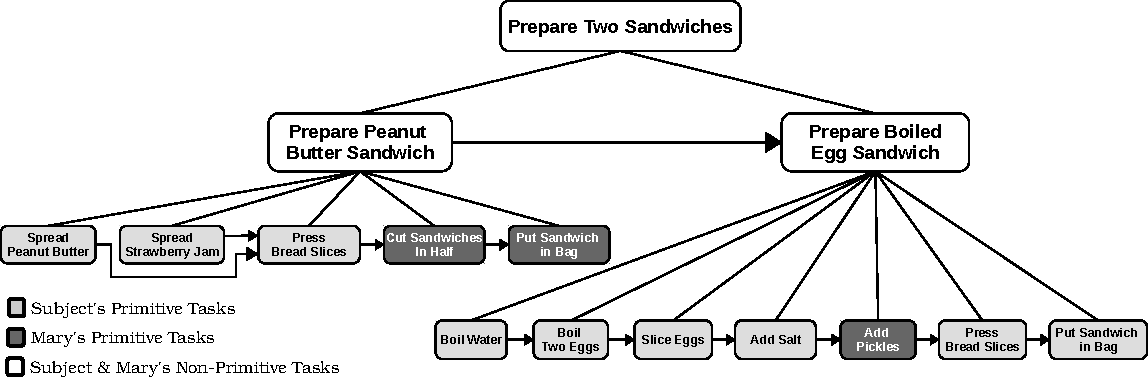
\includegraphics[width=12cm,height=4.25cm]{figure/taskModel-croped.pdf}
  \caption{Collaboration Task Model for the Evaluation.}
  \label{fig:taskModel}
\end{figure*}

To minimize the background knowledge necessary for our test subjects, we used a
simple domestic example of preparing a peanut butter and jelly sandwich, and a
hard boiled egg sandwich for a hiking trip. We provided textual and graphical
instructions for both questionnaires; Figure \ref{fig:taskModel} shows the
corresponding task model. The instructions presented a sequence of hypothetical
collaborative tasks to be carried out by the test subject and an imaginary
friend, Mary, in order to accomplish their goal of preparing two sandwiches. We
also provided a simple definition and an example of each appraisal variable. The
collaboration structure and the instructions were the same for both
questionnaires. The questions introduced specific situations related to the
shared plan, which included blocked tasks and failure or achievement of a shared
goal. Each question provided three answers which were counterbalanced in the
questionnaire. We provided an option like C in all questions, because we did not
want to force subjects to choose between two options when they did not have a
good reason. There were two questions designed based on each factor that we use
in our algorithms (see Section \ref{sec:appraisal}). The questions were
randomly placed in the questionnaire. Figure \ref{fig:qs1} shows an example
question from the relevance questionnaire which was designed to test whether
human subjects perceive saliency as a factor in relevance. The input for our
algorithms was the task model depicted in Figure \ref{fig:taskModel}.

\vspace*{-6mm}
\begin{table}[htbp]
\centering
\centering
\caption{Evaluation Results}
\begin{tabular}{|c|c|c|c|c|} \hline
appraisal variables & \# of subjects & mean & stdev & \textit{p}-value\\ \hline 
Relevance &  29 & 0.713 & 0.107 & $<$0.001\\ \hline
Desirability & 35 & 0.778 & 0.150 & $<$0.001\\ \hline 
Expectedness & 33 & 0.785 & 0.120 & $<$0.001\\ \hline 
Controllability & 33 & 0.743 & 0.158 & $<$0.001\\ \hline
\end{tabular}
\label{tbl:statistics}
\end{table}
\vspace*{-4mm}

Average results and standard deviation of the fractions of subjects' answers
agreeing with our algorithms output for both questionnaires are presented in
Table \ref{tbl:statistics}. Each question had 3 answers. Therefore, a random
distribution would result in 33\% agreement with our algorithms' output.
However, the average ratio indicating similarity between human subjects
decisions and the output of our algorithms is significantly higher than 33\%.
The total number of subjects' answers similar to the \textit{relevance}
algorithm (n=29) averaged 71.3\% (s=10.7\%), the \textit{desirability}
algorithm (n=35) averaged 77.8\% (s=15.0\%), the \textit{expectedness}
algorithm (n=33) averaged 78.5\% (s=12.0\%), and the \textit{controllability}
algorithm (n=33) averaged 74.3\% (s=15.8\%). It is worth noting that the human
subjects agreed 100\% on some questions, while on some other questions there
was a much lower level of agreement. Our results indicate that people largely
performed as our hypothesis predicted. The \textit{p}-values obtained based on a
one-tailed z-test (see Table \ref{tbl:statistics}) show the probability of human
subjects' answers being generated from a random set. The very small
\textit{p}-values indicate that the data set is not random; in fact, the high
percentage of similarity confirms our hypothesis and shows that the algorithms
can help us to model appraisal in a collaboration.

\begin{figure}[t]
  \vspace{-1mm}
  \centering
  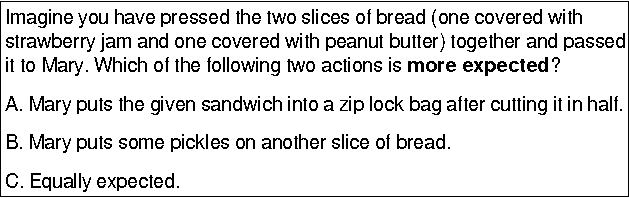
\includegraphics[width=0.8\textwidth]{figure/question-sample-croped.pdf}
  \caption{{\fontsize{9}{9}\selectfont Example Expectedness Question.}}
  \label{fig:qs1}
  \vspace{-2mm}
\end{figure}

Each question was designed based on different factors that we use in our
algorithms (see Section \ref{sec:appraisal}). Here, we present three
example questions from the expectedness, controllability, and desirability
questionnaires, and describe how each question relates to a specific factor
within the corresponding algorithm. The input for our algorithms was the task
model depicted in Figure \ref{fig:taskModel}.

Figure \ref{fig:qs1} shows the example question from the expectedness
questionnaire. In this example, with respect to Algorithm
\ref{alg:expectedness} (line 6), option A is more expected because the task
related to this option provides the next available task in the focus stack (see
the task model in Figure \ref{fig:taskModel}). Although the task in option B is
part of the existing task model, it is considered as unexpected by our
algorithm, since it is not live in the plan. We provided option C to determine
whether the human subjects will similarly differentiate between these two
options. This question was presented to the human subjects to determine whether
their decision for the expectedness of this event is similar to the output of
the expectedness algorithm. For this question, the human decision was 97\%
similar to the algorithm's output. Average results for the expectedness
questionnaire are presented in Table \ref{tbl:statistics}.

\begin{figure}[tbh]
  \vspace{-1mm}
  \centering
  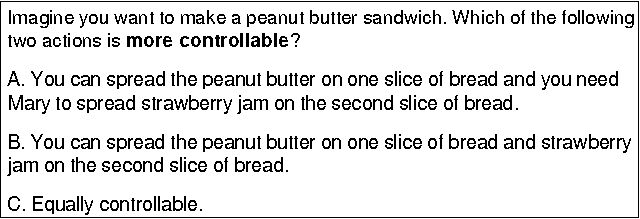
\includegraphics[width=0.8\textwidth]{figure/question-sample2-croped.pdf}
  \caption{{\fontsize{9}{9}\selectfont Example Controllability Question.}}
  \label{fig:qs2}
  \vspace{-2mm}
\end{figure}

Figure \ref{fig:qs2} shows an example question from the controllability
questionnaire. The algorithm's output is option B, and is determined by
Algorithm \ref{alg:controllability} (line 3), similarly to the expectedness
example above. In this example, option B is more controllable than option A,
because the self over total ratio of the responsibility of the predecessors of
the given task (see \textit{Autonomy} in Section \ref{sec:controllability}) is
higher than the ratio in option A; i.e., self is responsible to spread peanut
butter on one slice of bread and strawberry jam on another slice of bread. In
this question, the humans decision was 90\% in agreement with the algorithm's
output.

\begin{figure}[t]
  \vspace{-1mm}
  \centering
  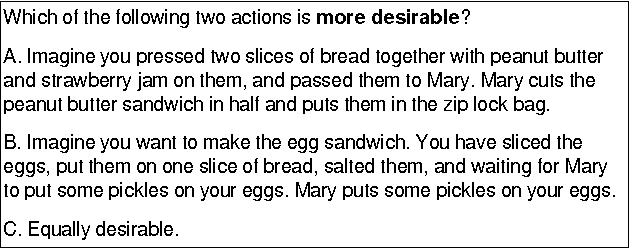
\includegraphics[width=0.8\textwidth]{figure/question-sample3-croped.pdf}
  \caption{{\fontsize{9}{9}\selectfont Example Desirability Question.}}
  \label{fig:qs3}
  \vspace{-2mm}
\end{figure}

Figure \ref{fig:qs3} shows an example question from the desirability
questionnaire. The output based on the Algorithm \ref{alg:desirability}
(line 14) is option C, since in both option A and option B, the focus goal
has been achieved successfully. Therefore, in this example, both options A and B
are desirable. The humans decision was 77\% in agreement with the algorithm's
output in this question.

\begin{figure}[tbh]
  \vspace{-1mm}
  \centering
  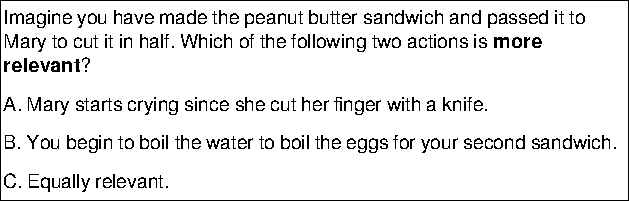
\includegraphics[width=0.8\textwidth]{figure/question-sample4-croped.pdf}
  \caption{{\fontsize{9}{9}\selectfont Example Relevance Question.}}
  \label{fig:qs4}
  \vspace{-2mm}
\end{figure}

In the example shown in Figure \ref{fig:qs4}, with respect to Algorithm
\ref{alg:relevance}, option A is relevant because of Mary's perceived negative
emotion (see Equation \ref{eqn:utility}). Although option B is relevant (since
it achieves the next goal in the shared plan), 83\% of subjects consider it as
less relevant than option A; we believe this is due to the effect of Mary's
perceived negative emotion which also generates higher utility value in our
relevance algorithm. Another question also tested belief saliency. However, the
options provided only related to the shared plan (i.e., no human emotions in the
options). In this case 87\% of subjects chose the option that accomplished the
next goal in the shared plan. Interestingly, when confronted with a negative
emotion from their collaborator, human subjects deviated from the shared plan
and found their collaborator's emotion more relevant than the original plan. It
is noteworthy that in both the absence and the presence of emotions the human
subjects chose the more salient option with respect to our definition of
saliency, which was not referenced or provided in the questionnaire.

Furthermore, as we mentioned earlier, there were two questions related to each
factor in our algorithms. Because each question was asking about a specific
factor, we were able to perform a sensitivity analysis, similar to the saliency
example presented above. We observed similar results for other factors of both
relevance (e.g., persistence) and controllability (e.g., autonomy), but do not
present them here due to space constraints.

\section{Conclusion and Future Work}

There is a correspondence between what a collaboration needs and the social
functions of emotions. In this paper, we presented a theory explaining the
processes underlying in collaboration using social emotions. We provided four
hypothetical examples in two pairs, each dealing with an important collaborative
behavior. The first pair was about agreeing on a shared goal; the second pair
was about delegation of a new task. Each pair of examples contrasted a
successful collaboration, due to the Robot's awareness of the Astronaut's
emotion, with a failure in collaboration, due to the Robot's ignorance of the
Astronaut's emotions. These examples illustrated the importance of
emotional awareness to attain successful collaborative behavior.

We then introduced the main components of Affective Motivational Collaboration
Theory, our computational framework which integrates emotion-regulated
mechanisms, such as appraisal and coping, with collaboration processes, such as
planning, in a single unified framework. This framework will let us to explain
the collaborative processes in computational detail.

As shown in this paper, there are factors involved in appraisal processes
that are not accounted for in existing appraisal models. These factors,
including the influence of the human collaborator's emotions must be addressed
to provide proper collaborative behavior in a robot. The SharedPlans theory and
other computational collaboration theories (e.g., Joint Intentions) emphasize
the importance of commitment in collaboration. According to these theories
collaborators are required to commit to their shared plan or intentions to
successfully collaborate and achieve a shared goal. This commitment requires
them to appraise their environment based on the shared plan structure, as well
as other information that is induced by the collaboration process, such as the
recurrence of a belief by the other collaborator and the human collaborator's
perceived emotion. In our next step, we want to test our appraisal algorithms
and their reciprocal influence on goal management during collaboration. This
study will be conducted between a KUKA youbot and human subjects on a different
task model.

% We have started to implement the rules associated with these computational
% walkthroughs using JESS (Java Expert System Shell) which is a rule engine for
% the Java platform. In our current implementation we have categorized the rules
% into different modules associated with the mechanisms and the processes in
% Affective Motivational Collaboration Theory. In our future work, we will
% implement complete algorithms for each mechanism and process, thereby automating
% the computational walkthroughs. Our ultimate goal is a general software platform
% based on the collaboration structure of SharedPlans theory
% \cite{grosz:discourse-structure}, and employing emotion-driven processes such as
% appraisal \cite{marsella:ema-process-model} to enable a robot to employ
% emotion-regulated collaborative behaviors in its interactions with humans.

%\label{sec:2} ~\ref{sec:1}

%\paragraph{Paragraph headings} 


% For one-column wide figures use
%\begin{figure}
% Use the relevant command to insert your figure file.
% For example, with the graphicx package use
%  
\includegraphics{example.eps}
% figure caption is below the figure
%\caption{Please write your figure caption here}
%\label{fig:1}       % Give a unique label
%\end{figure}
%
% For two-column wide figures use
%\begin{figure*}
% Use the relevant command to insert your figure file.
% For example, with the graphicx package use
%  
\includegraphics[width=0.75\textwidth]{example.eps}
% figure caption is below the figure
%\caption{Please write your figure caption here}
%\label{fig:2}       % Give a unique label
%\end{figure*}
%



% For tables use
%\begin{table}
% table caption is above the table
%\caption{Please write your table caption here}
%\label{tab:1}       % Give a unique label
% For LaTeX tables use
%\begin{tabular}{lll}
%\hline\noalign{\smallskip}
%first & second & third  \\
%\noalign{\smallskip}\hline\noalign{\smallskip}
%number & number & number \\
%number & number & number \\
%\noalign{\smallskip}\hline
%\end{tabular}
%\end{table}


%\begin{acknowledgements}
%If you'd like to thank anyone, place your comments here
%and remove the percent signs.
%\end{acknowledgements}

% BibTeX users please use one of
%\bibliographystyle{spbasic}      % basic style, author-year citations
%\bibliographystyle{spmpsci}      % mathematics and physical sciences
%\bibliographystyle{spphys}       % APS-like style for physics
%\bibliography{}   % name your BibTeX data base

% Non-BibTeX users please use
%\begin{thebibliography}{}
%
% and use \bibitem to create references. Consult the Instructions
% for authors for reference list style.
%
%\bibitem{RefJ}
% Format for Journal Reference
%Author, Article title, Journal, Volume, page numbers (year)

% Format for books

%\bibitem{RefB}
%Author, Book title, page numbers. Publisher, place (year)

% etc
%\end{thebibliography}

\bibliographystyle{abbrv}
\bibliography{mshayganfar.bib}

\end{document}
% end of file template.tex

